\documentclass{article}
\usepackage[margin=1in]{geometry}
\usepackage[utf8]{inputenc}
\usepackage{amsfonts,amsmath,bm}
\usepackage{xcolor}
\usepackage{graphicx}
\usepackage{caption}
\usepackage{subcaption}
\usepackage{tabulary}
\usepackage{multirow}
\usepackage{algorithm}
\usepackage{algpseudocode}
\usepackage{hyperref}
% color def
\usepackage{color}
\definecolor{darkred}{rgb}{0.6,0.0,0.0}
\definecolor{darkgreen}{rgb}{0,0.50,0}
\definecolor{lightblue}{rgb}{0.0,0.42,0.91}
\definecolor{orange}{rgb}{0.99,0.48,0.13}
\definecolor{grass}{rgb}{0.18,0.80,0.18}
\definecolor{pink}{rgb}{0.97,0.15,0.45}

% listings
\usepackage{listings}

% General Setting of listings
\lstset{
  aboveskip=1em,
  breaklines=true,
  abovecaptionskip=-6pt,
  captionpos=b,
  escapeinside={\%*}{*)},
  frame=single,
  numbers=left,
  numbersep=15pt,
  numberstyle=\tiny,
}
% 0. Basic Color Theme
\lstdefinestyle{colored}{ %
  basicstyle=\ttfamily,
  backgroundcolor=\color{white},
  commentstyle=\color{green}\itshape,
  keywordstyle=\color{blue}\bfseries\itshape,
  stringstyle=\color{red},
}
% 1. General Python Keywords List
\lstdefinelanguage{PythonPlus}[]{Python}{
  morekeywords=[1]{,as,assert,nonlocal,with,yield,self,True,False,None,} % Python builtin
  morekeywords=[2]{,__init__,__add__,__mul__,__div__,__sub__,__call__,__getitem__,__setitem__,__eq__,__ne__,__nonzero__,__rmul__,__radd__,__repr__,__str__,__get__,__truediv__,__pow__,__name__,__future__,__all__,}, % magic methods
  morekeywords=[3]{,object,type,isinstance,copy,deepcopy,zip,enumerate,reversed,list,set,len,dict,tuple,range,xrange,append,execfile,real,imag,reduce,str,repr,}, % common functions
  morekeywords=[4]{,Exception,NameError,IndexError,SyntaxError,TypeError,ValueError,OverflowError,ZeroDivisionError,}, % errors
  morekeywords=[5]{,ode,fsolve,sqrt,exp,sin,cos,arctan,arctan2,arccos,pi, array,norm,solve,dot,arange,isscalar,max,sum,flatten,shape,reshape,find,any,all,abs,plot,linspace,legend,quad,polyval,polyfit,hstack,concatenate,vstack,column_stack,empty,zeros,ones,rand,vander,grid,pcolor,eig,eigs,eigvals,svd,qr,tan,det,logspace,roll,min,mean,cumsum,cumprod,diff,vectorize,lstsq,cla,eye,xlabel,ylabel,squeeze,}, % numpy / math
}
% 2. New Language based on Python
\lstdefinelanguage{PyBrIM}[]{PythonPlus}{
  emph={d,E,a,Fc28,Fy,Fu,D,des,supplier,Material,Rectangle,PyElmt},
}
% 3. Extended theme
\lstdefinestyle{colorEX}{
  basicstyle=\ttfamily,
  backgroundcolor=\color{white},
  commentstyle=\color{darkgreen}\slshape,
  keywordstyle=\color{blue}\bfseries\itshape,
  keywordstyle=[2]\color{blue}\bfseries,
  keywordstyle=[3]\color{grass},
  keywordstyle=[4]\color{red},
  keywordstyle=[5]\color{orange},
  stringstyle=\color{darkred},
  emphstyle=\color{pink}\underbar,
}
% \usepackage{biblatex}
% \addbibresource{bibliography.bib} %Import the bibliography file
% \usepackage[framed,numbered,autolinebreaks,useliterate]{mcode}
\usepackage{tikz}
\newcommand*\circled[1]{\tikz[baseline= (char.base)]{
            \node[shape=circle, draw, inner sep=1.5pt] (char) {#1};}}
\newcommand*\smallcircled[1]{\tikz[baseline= (char.base)]{
            \node[shape=circle, draw, inner sep=0.5pt] (char) {#1};}}


\title{EEC269A - Error Correcting Codes I\\Project Report}
\author{Chenye Yang, Pranav Kharche, Parisa Oftadeh}
\date{\today}

\begin{document}

\maketitle

\tableofcontents














\newpage
\section{Workload}

\begin{table}[htb]
    \centering
    \caption{Workload}
    \label{tab:workload}
    \renewcommand{\arraystretch}{1.5}
    \begin{tabulary}{\textwidth}{ |L|L|L| } 
    \hline
    \textbf{Function} & \textbf{Workload} & \textbf{Contributor} \\
    \hline
    Source & Text string (TXT), Image (PNG), Audio (WAV) & Chenye \\ 
    \hline
    \multirow{2}{*}{Encoder} & $(7,4)$ Systematic Linear Block (Hamming) Code & Chenye \\ 
    & $(n,k)$ Systematic Cyclic (Hamming) Code & Pranav, Chenye \\ 
    \hline
    \multirow{2}{*}{Channel} & Binary Symmetric Channel (BSC), error probability $p$ adjustable & Chenye \\ 
    & AWGN & Parisa \\ 
    \hline
    \multirow{3}{*}{Error Corrector} &  Syndrome Lookup Table for $(7,4)$ Linear Code & Chenye \\ 
    & Syndrome Lookup Table for $(n,k)$ Cyclic Code & Chenye \\ 
    & LFSR for $(n,k)$ Cyclic Code & Pranav \\
    \hline
    \multirow{2}{*}{Decoder} & $(7,4)$ Systematic Linear Block (Hamming) Code & Chenye \\ 
    & $(n,k)$ Systematic Cyclic (Hamming) Code & Chenye \\ 
    \hline
    Destination & Text string (TXT), Image (PNG), Audio (WAV) & Chenye \\ 
    \hline
    \multirow{2}{*}{\textbf{Advanced features}} & \textbf{Create generator matrix for $(n,k)$ cyclic code} & Pranav \\ 
    & \textbf{Adjustable $(n,k)$} & Pranav \\
    \hline
    \textbf{Presentation} & Slides & Parisa \\ 
    \hline
    \textbf{Report} & Written by contributors & - \\
    \hline
    \end{tabulary}
\end{table}



\section{Source \& Destination}
\subsection{Source}

\subsubsection{Text string}
The very basic function of the information source is to read a hard-coded text file into a bit stream. 
In our text file, the following string is stored in ASCII format:
\begin{center}
    Hello World!\\EEC269A Error Correcting Code Demo
\end{center}
In ASCII format, each character is represented by 8 bits, shown in Table~\ref{tab:ascii}. Then, after transformation, the bit stream is of size 376 bits: 
\begin{center}
    0 1 0 0 1 0 0 0 0 1 1 0 0 1 0 1 \dots
\end{center}

\begin{table}[ht]
    \centering
    \caption{ASCII Table example}
    \label{tab:ascii}
    \begin{tabulary}{\textwidth}{|L|L|L|L|}
    \hline
    Character & Hexadecimal & Decimal & Binary \\
    \hline
    \dots & \dots & \dots & \dots \\
    \hline
    A & 41 & 65 & 0 1 0 0 0 0 0 1 \\
    \hline
    B & 42 & 66 & 0 1 0 0 0 0 1 0 \\
    \hline
    C & 43 & 67 & 0 1 0 0 0 0 1 1 \\
    \hline
    D & 44 & 68 & 0 1 0 0 0 1 0 0 \\
    \hline
    E & 45 & 69 & 0 1 0 0 0 1 0 1 \\
    \hline
    F & 46 & 70 & 0 1 0 0 0 1 1 0 \\
    \hline
    G & 47 & 71 & 0 1 0 0 0 1 1 1 \\
    \hline
    H & 48 & 72 & 0 1 0 0 1 0 0 0 \\
    \hline
    \dots & \dots & \dots & \dots \\
    \hline
    \end{tabulary}
\end{table}


\subsubsection{Image}
PNG (Portable Network Graphics) is a raster graphics file format that supports lossless data compression. 
PNG supports a large number of colors (up to 16 million), as well as variable transparency, which makes it useful for images with varying degrees of transparency or opacity. 
Additionally, because PNG is a lossless format, it preserves all the detail in the original image, which is not the case with lossy formats like JPEG. 
It is used for the storage and display of images on the internet, and is also used in graphic design and editing applications due to its lossless compression.

PNG files consist of a header followed by a series of data chunks, e.g.:
\begin{enumerate}
    \item Signature: The first eight bytes of a PNG file always contain the following decimal numbers: 137, 80, 78, 71, 13, 10, 26, 10. This signature indicates that the file is a PNG.
    \item Header Chunk (IHDR): The first chunk after the signature is the IHDR chunk, which contains basic information about the image, such as width, height, bit depth, color type, compression method, filter method, and interlace method.
    \item Palette Chunk (PLTE): This chunk is optional and only present for color type 3 (indexed color). It contains the color palette for the image.
    \item Data Chunks (IDAT): These chunks contain the actual image data, which is formed by pixels. This data is compressed to reduce the size of the file.
    \item End Chunk (IEND): This is the final chunk in a PNG file. It does not contain any data and its purpose is to indicate the end of the file.
\end{enumerate}
Each chunk contains three standard fields: 4-byte length, 4-byte type code, 4-byte CRC and various internal fields that depend on the chunk type, shown in Figure~\ref{fig:png-structure} \footnote{Figure~\ref{fig:png-structure} is from webpage \href{https://www.nayuki.io/res/dumb-png-output-java/png-file-format.svg}{PNG file chunk inspector - Project Nayuki}}. 
For example, the image file we are using has more than one image data (IDAT) chunks, each of which contains a portion of the image, shown in Table~\ref{tab:our-png-structure}.

\begin{figure}[htb]
    \centering
    \hfill
    \begin{minipage}[b]{0.3\textwidth}
        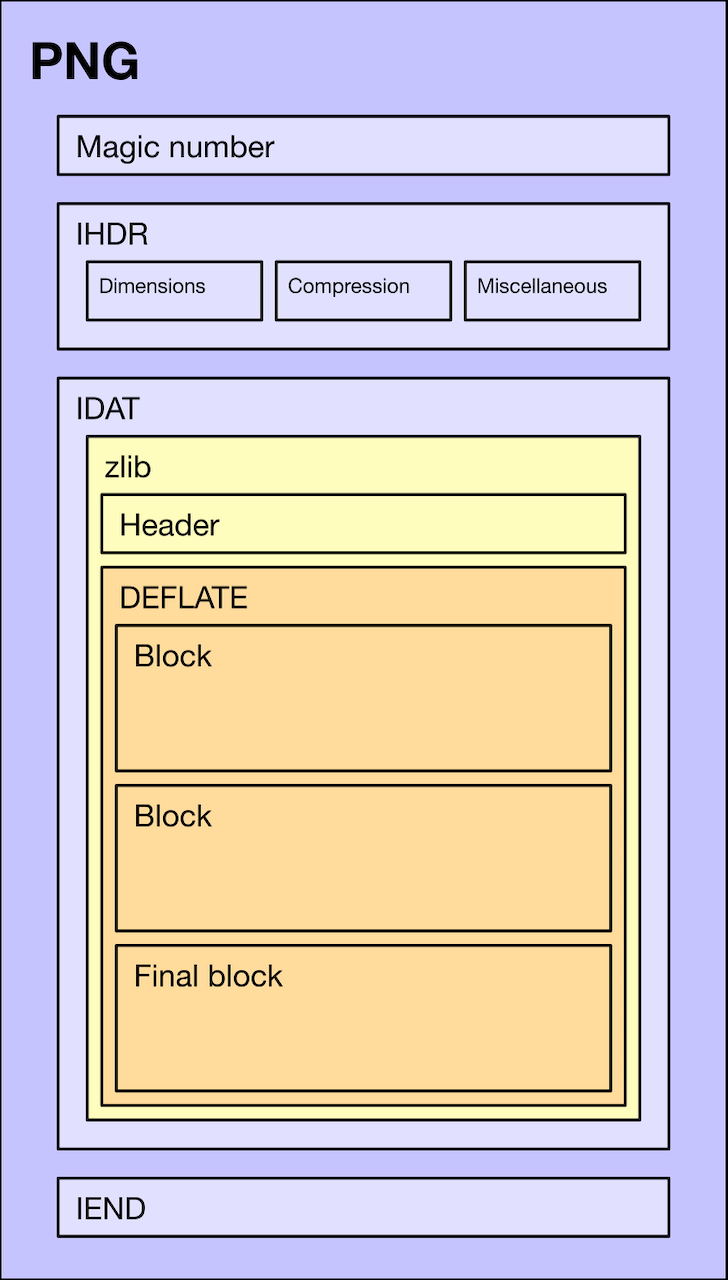
\includegraphics[width=\textwidth]{png-file-format.png}
        \caption{PNG file structure}
    \label{fig:png-structure}
    \end{minipage}
    \hfill
    \begin{minipage}[b]{0.36\textwidth}
        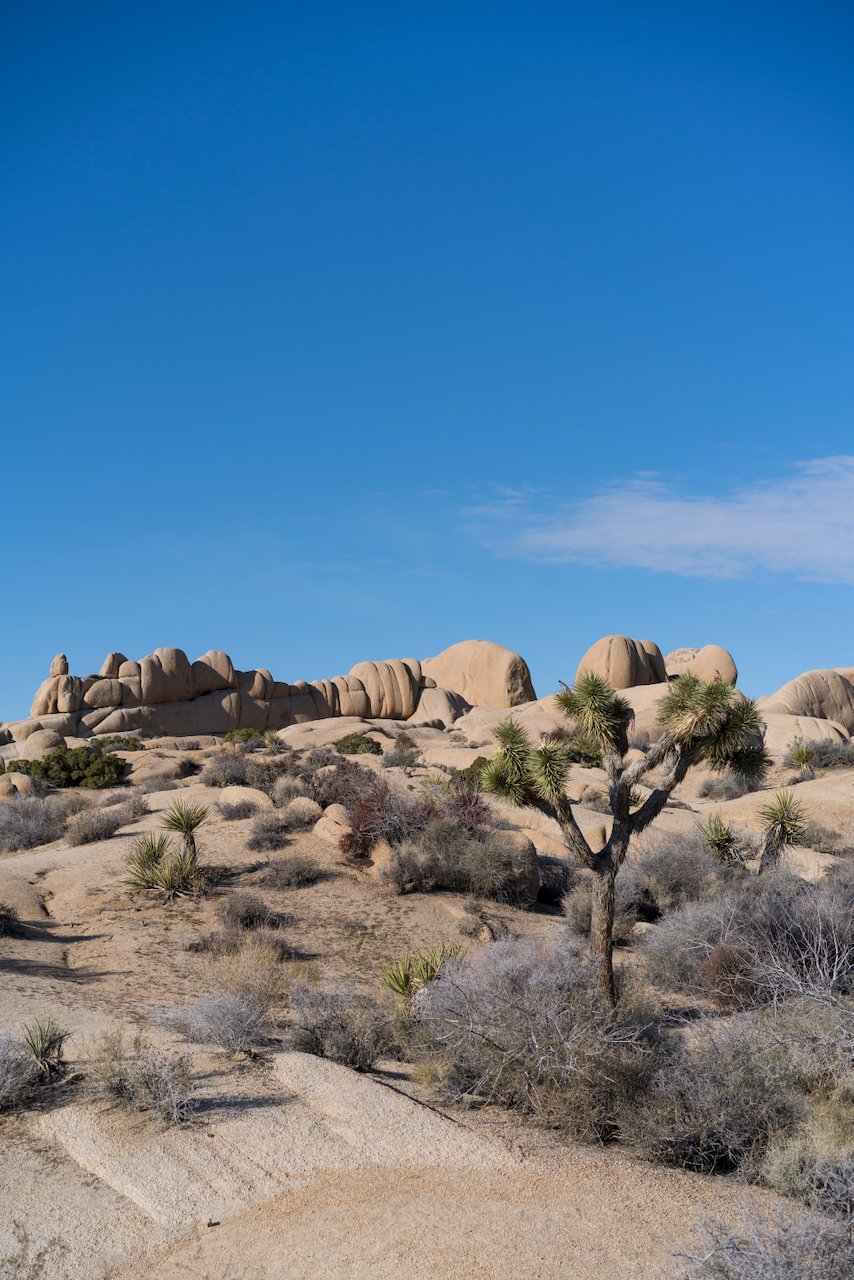
\includegraphics[width=\textwidth]{../Resource/image.png}
        \caption{Our testing PNG image}
    \label{fig:our-image}
    \end{minipage}
    \hfill
\end{figure}


\begin{table}[htb]
    \centering
    \caption{Our PNG file structure}
    \label{tab:our-png-structure}
    \renewcommand{\arraystretch}{1.5}
    \begin{tabulary}{\textwidth}{ |L|L| } 
    \hline
    Start offset & Chunk outside \\
    \hline
    0 & Special: File signature; Length: 8 bytes \\
    \hline
    8 & Data length: 13 bytes; Type: IHDR; Name: Image header; CRC-32: CB3954EC \\
    \hline
    33 & Data length: 1 bytes; Type: sRGB; Name: Standard RGB color space; CRC-32: AECE1CE9 \\
    \hline
    46 & Data length: 976 bytes; Type: eXIf; Name: Exchangeable Image File (Exif) Profile; CRC-32: 47FCFA4D \\
    \hline
    1,034 & Data length: 9 bytes; Type: pHYs; Name: Physical pixel dimensions; CRC-32: 5024E7F8 \\
    \hline
    1,055 & Data length: 4 514 bytes; Type: iTXt; Name: International textual data; CRC-32: C9C76B16 \\
    \hline
    5,581 & Data length: 16 384 bytes; Type: IDAT; Name: Image data; CRC-32: 8462CABD \\
    \hline
    21,977 & Data length: 16 384 bytes; Type: IDAT; Name: Image data; CRC-32: 2C9D007C \\
    \hline
    \dots & \dots \\
    \hline
    1,727,161 & Data length: 12 170 bytes; Type: IDAT; Name: Image data; CRC-32: 68067F52 \\
    \hline
    1,739,343 & Data length: 0 bytes; Type: IEND; Name: Image trailer; CRC-32: AE426082 \\
    \hline
    \end{tabulary}
\end{table}

Ideally, the entire image file should be read into a bit stream and transmitted through the channel. 
However, if there are uncorrectable errors in the chunks other than the image data (IDAT), the received image will not be able to display.
Therefore, we shall only work with the image data (IDAT) chunks for the purpose of visualization of a corrupted image. 
Also, this trick will not affect the statistical analysis of the system. 

The information source is able to only extract the color information from a PNG file and convert it into a bit stream to be passed through the channel. 
This is done by using the Python library \textit{NumPy}.

The library \textit{NumPy} provides a method to only read out the color information of an image. The shape of the result array is typically \textit{(height, width, channels)}, where:
\begin{enumerate}
    \item \textit{height} is the number of pixels in the vertical direction (i.e. the number of rows of pixels);
    \item \textit{width} is the number of pixels in the horizontal direction (i.e. the number of columns of pixels);
    \item \textit{channels} is the number of color channels per pixel. This value depends on what type of image it is: \begin{itemize}
        \item In an RGB image, the three channels correspond to Red, Green, and Blue, respectively. Each channel value usually ranges from 0 to 255, where 0 indicates none of that color is present and 255 indicates that color is fully present.
        \item In a grayscale image, there is typically only one channel. The value in this single channel indicates the level of gray, where 0 is black and 255 is white.
        \item There are many other color spaces that have different meanings for their channels.
    \end{itemize}
\end{enumerate}
The data type for each channel of each pixel is \textit{uint8}, which is an unsigned integer that takes 8 bits.
Then, the array is flattened into a bit stream by converting each channel of each pixel into an 8-bits binary number and appending them together.

For example, as for our testing image\footnote{The image file used in this project is photographed by \textit{Chenye Yang}. The material is free from any copyright restrictions and can be used without any potential legal implications.}, shown in Figure~\ref{fig:our-image}, the shape of the result array is \textit{(1280, 854, 3)}, which means that the image has 1280 rows of pixels, 854 columns of pixels, and 3 color channels per pixel (RGB). 
Then, the array is flattened into a bit stream of 26,234,880 bits.







\subsubsection{Audio}
WAV (Waveform Audio File Format) is a digital audio standard for storing audio bitstream on PCs. 
WAV is an application of the Resource Interchange File Format (RIFF) method for storing data in chunks, and it is primarily used on Windows systems. 
WAV files are typically used for raw and uncompressed audio, though they can also contain compressed audio.
A WAV file is divided into several sections or chunks, shown in Figure~\ref{fig:canonical-wav-structure} \footnote{Figure~\ref{fig:canonical-wav-structure} is from webpage \href{https://www.videoproc.com/resource/wav-file.htm}{WAV Files: File Structure, Case Analysis and PCM Explained}}. Each chunk serves a different purpose and holds different types of data. The basic structure of a WAV file includes the following chunks:
\begin{enumerate}
    \item RIFF Chunk: The RIFF chunk is the first chunk in a WAV file and identifies the file as a WAV file. It includes a header with the "RIFF" identifier and an integer indicating the remaining length of the entire file.
    \item Format Chunk: Also known as the "fmt " chunk (with a space after 'fmt'), this contains important information about the audio data. This includes the audio format (e.g., PCM), the number of channels (mono, stereo, etc.), the sample rate, the byte rate, the block alignment, and the bit depth (bits per sample).
    \item Data Chunk: This is where the actual audio data is stored. The "data" header is followed by an integer representing the length of the data, and then by the raw audio data itself.
\end{enumerate}


\begin{figure}[htb]
    \centering
    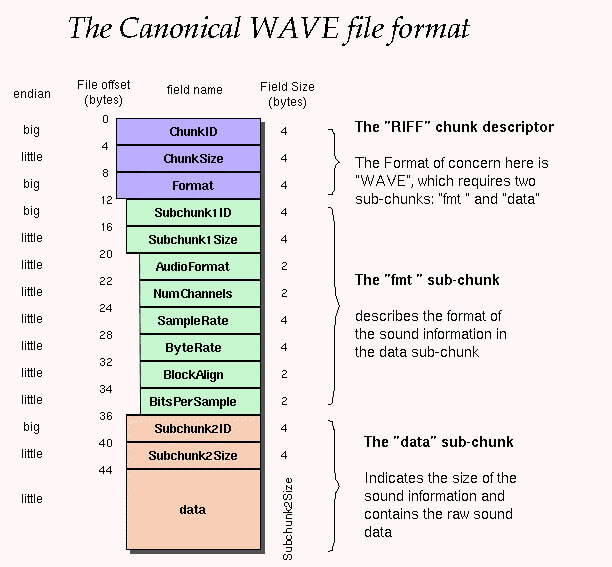
\includegraphics[width=0.7\textwidth]{canonical-wav-file-structure.jpg}
    \caption{Canonical WAV file structure}
    \label{fig:canonical-wav-structure}
\end{figure}

Similar to the image file, the information source is able to only extract the audio Data Chunk from a WAV file and convert it into a bit stream to be passed through the channel. 
This trick ensures both the visualization of the results and the statistical analysis of the system. The extraction is done by using the Python library \textit{soundfile}.

The library \textit{soundfile} provides a method to only read out the audio data from a WAV file. The result contains two parts:
\begin{enumerate}
    \item audio array: This is a \textit{NumPy} array that contains the audio data from the file. The shape of the array depends on the number of channels in the audio file. If the audio is mono, the array will be one-dimensional. If the audio is stereo, the array will be two-dimensional, with one sub-array for each channel. The values in the array represent the amplitude of the audio signal at each sample point, and are of the data type specified.
    \item sample rate: This is an integer that represents the number of samples per second in the audio file, measured in Hertz (Hz). Common sample rates include 44100 Hz (standard for audio CDs), 48000 Hz (standard for video production and DVDs), and 96000 Hz (used in high-definition formats).
\end{enumerate}
Then, the \textit{int16} array is "viewed" as \textit{uint8} array by \textit{numpy.view()} and flattened into a bit stream by converting each sample into an 8-bits binary number and appending them together. 
Note that the \textit{numpy.view()} operation simply reinterprets the binary data, and does not convert or scale the data, which originally could be negative or positive. 

For example, as for our testing audio file\footnote{The audio file used in this project is free downloaded from \href{https://file-examples.com/index.php/sample-audio-files/sample-wav-download/}{file-examples.com}. The material is free from any copyright restrictions and can be used without any potential legal implications.}, shown in Figure~\ref{fig:our-audio-time-domain} and Figure~\ref{fig:our-audio-frequency-domain}, 
the shape of the result audio array is \textit{(268237, 2)} and the sample rate is 8000 Hz. It means that the 33.5-second audio file has 268237 samples per channel, and there are two channels (stereo). 
Then, the array is flattened into a bit stream of 8,583,584 bits.


\begin{figure}[htb]
    \centering
    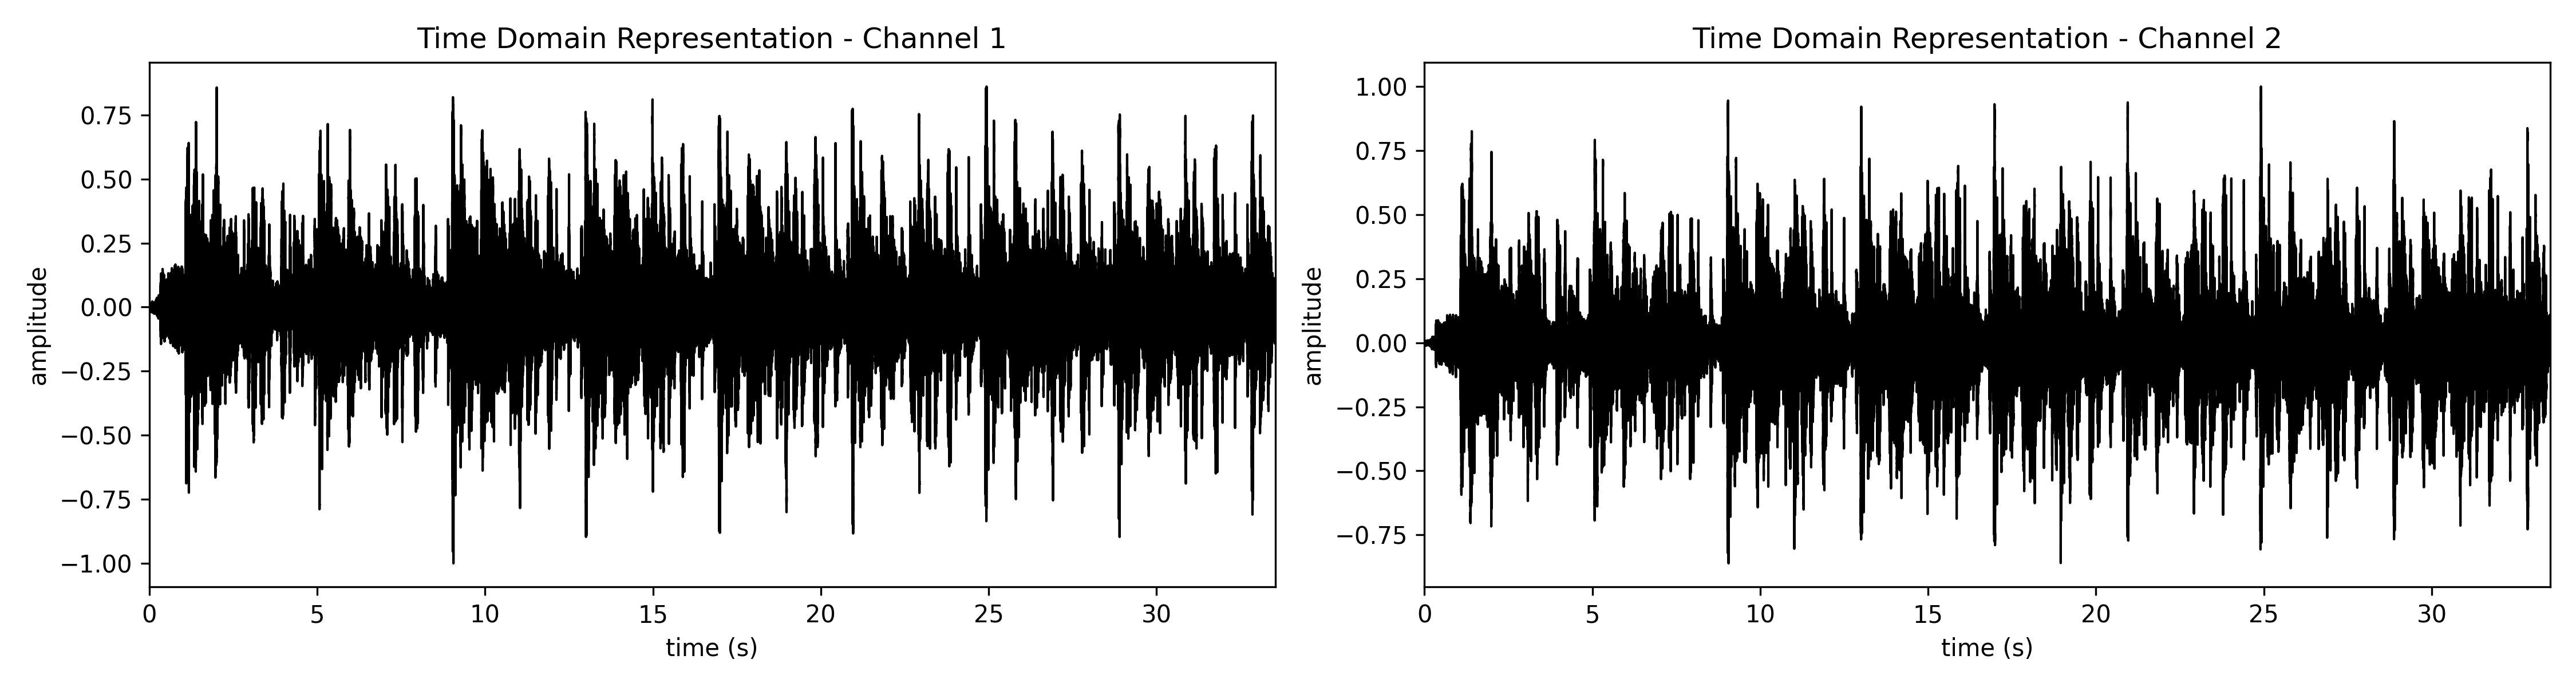
\includegraphics[width=\textwidth]{../Result/wav-time-domain-TX.png}
    \caption{Time domain waveform of our testing audio file}
    \label{fig:our-audio-time-domain}
\end{figure}

\begin{figure}[htb]
    \centering
    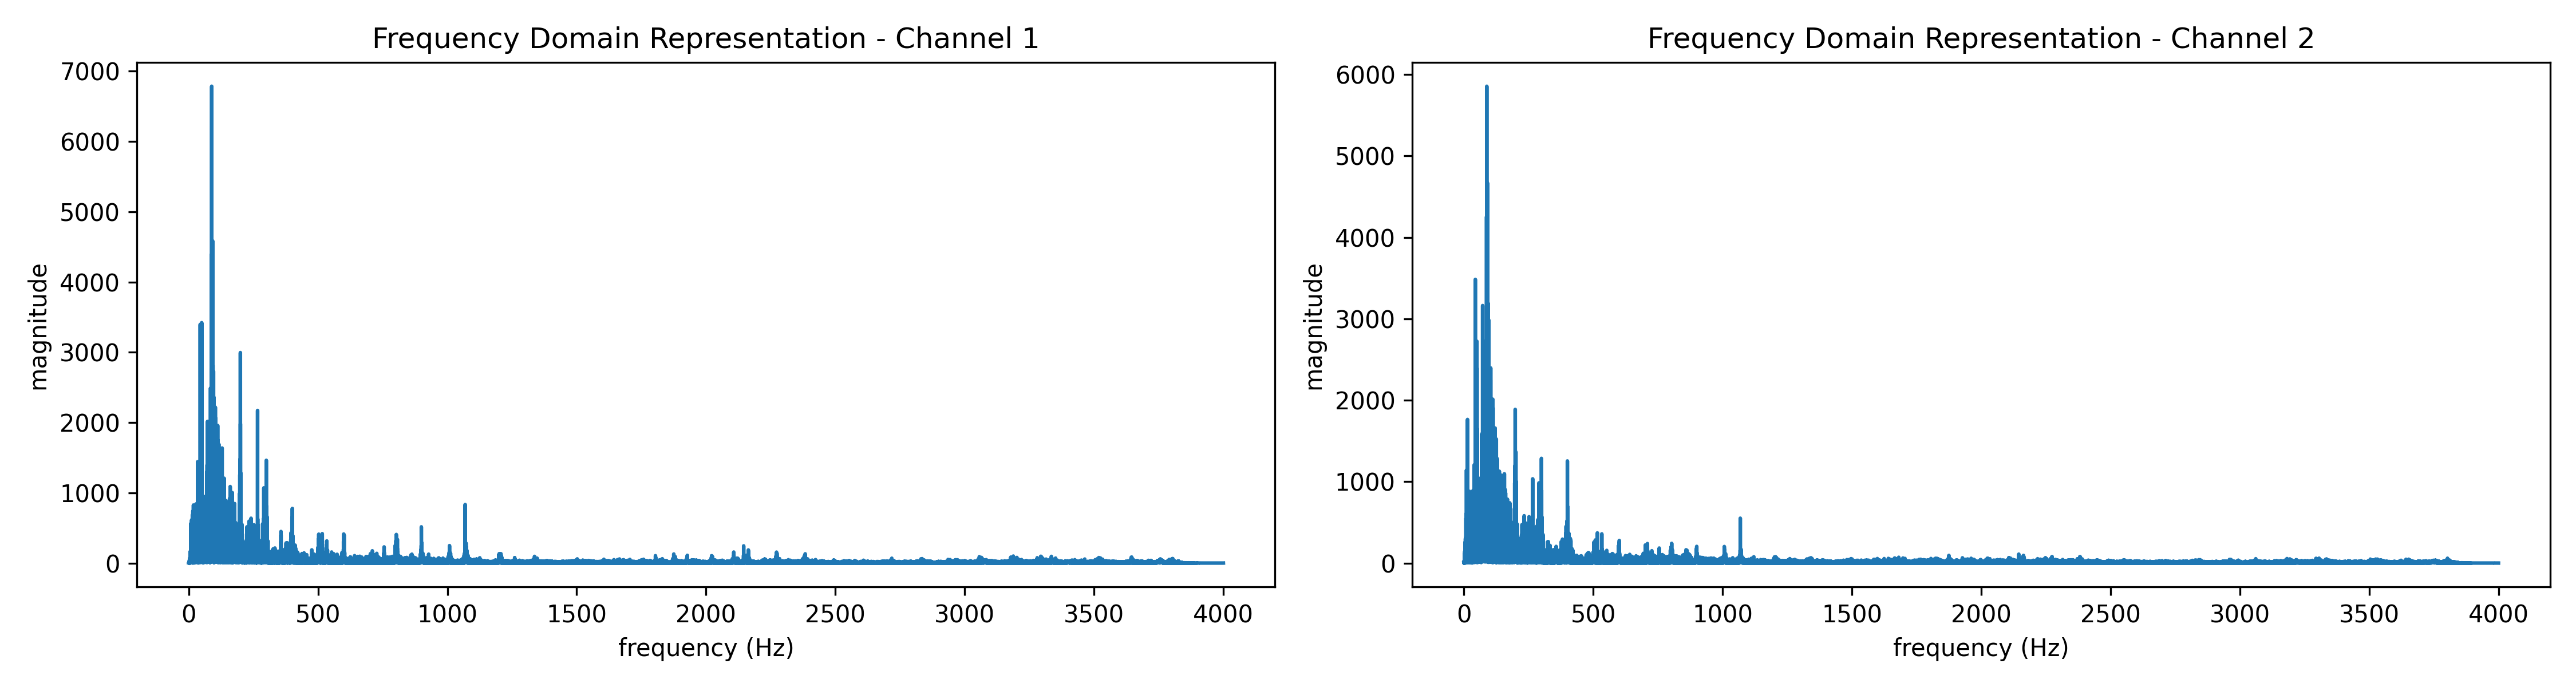
\includegraphics[width=\textwidth]{../Result/wav-frequency-domain-TX.png}
    \caption{Frequency domain waveform of our testing audio file}
    \label{fig:our-audio-frequency-domain}
\end{figure}







\subsection{Destination}
At the destination, the bit stream is re-construed into the original format, and stored. 
It is inevitable that some metadata is lost when processed by the system, since they are not transmitted through the channel.
For example, the re-constructed image file will not have the camera and lens information. 
However, this is the trade-off for a better visualization, and will not affect the statistical analysis of the system.








\section{Channel}

\subsection{Binary Symmetric Channel (BSC)}
The Binary Symmetric Channel (BSC) is a fundamental concept in information theory and telecommunications, specifically in the field of error detection and correction. It is a model used to represent a communication channel, where the information is transmitted in the form of binary digits, or bits: 0s and 1s.

The "symmetric" aspect of the BSC refers to the fact that it has the same probability of an error occurring whether the transmitted bit is a 0 or a 1. For instance, if the error probability is 0.01, then 1\% of 0s are received as 1s, and 1\% of 1s are received as 0s. 

A BSC is characterized by two parameters: the input bit and the crossover probability / error probability, shown in Figure~\ref{fig:bsc}. The input bit is either 0 or 1, which represents the binary information being transmitted. The crossover probability, often denoted as $p$, represents the likelihood of the transmitted bit being received incorrectly. 

Although the model is simple, the BSC is a building block for understanding more complex communication systems. By studying the BSC, researchers can develop algorithms and systems that minimize errors in binary data transmission, improving the reliability of digital communications.

\begin{figure}[htb]
    \centering
    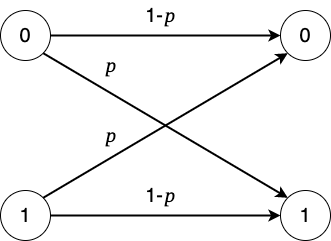
\includegraphics[width=0.3\textwidth]{bsc.png}
    \caption{Binary Symmetric Channel (BSC)}
    \label{fig:bsc}
\end{figure}








\subsection{Additive White Gaussian Noise (AWGN) Channel}










\section{(7,4) Systematic Linear Block (Hamming) Code}
The (7,4) Systematic Linear Block (Hamming) Code, often referred to simply as the Hamming (7,4) Code, is a fundamental concept in the realm of error detection and correction, and plays a crucial role in the field of digital communications and information theory. This coding scheme was introduced by Richard Hamming in the late 1940s to address the problem of error detection and correction in data transmission over noisy channels.

The Hamming (7,4) Code is a block code that maps 4-bit messages to 7-bit codewords. It gets its name from the fact that it takes in 4 data bits and outputs 7 bits (including 3 parity bits). The parity bits are extra bits added to the data to enable the detection and correction of errors that might occur during transmission.

A key characteristic of the Hamming (7,4) Code is its systematic form. This means that the bits of the original message appear unaltered in the encoded output, making it easy to extract the original data from the received message, even if errors are detected. 

The Hamming (7,4) Code is designed to detect and correct single-bit errors, meaning it can identify and fix any situation where only one bit in the 7-bit codeword has been flipped due to noise or interference in the communication channel. This makes it a powerful tool in improving the reliability and robustness of data communication systems.



\subsection{Encoder}
The encoding process in a Hamming (7,4) code involves the multiplication of a 4-bit message vector with a generator matrix. The generator matrix for a (7,4) Hamming Code, in its systematic form, is given as:
\begin{equation*}
    G = 
        \begin{bmatrix}
        1 & 1 & 0 & 1 & 0 & 0 & 0 \\
        0 & 1 & 1 & 0 & 1 & 0 & 0 \\
        1 & 1 & 1 & 0 & 0 & 1 & 0 \\
        1 & 0 & 1 & 0 & 0 & 0 & 1 \\
        \end{bmatrix}.
\end{equation*}
If we denote the message vector as 
\begin{equation*}
    u =
        \begin{bmatrix}
        u_1 & u_2 & u_3 & u_4 
        \end{bmatrix},
\end{equation*}
then the encoded codeword $v$ is computed by:
\begin{equation*}
    v = u \cdot G .
\end{equation*}
This multiplication produces a 7-bit codeword, which is then ready for transmission.





\subsection{Syndrome Decoder}
The decoding process of the (7,4) Hamming code involves utilizing a syndrome lookup table. The syndrome, a binary vector, is computed from the received bits and is used to identify the error bit position. Each syndrome corresponds to a potential error location, and its lookup table is a key tool for efficient error correction.





\subsubsection{Results: text string}

\begin{table}[htb]
    \centering
    \caption{Text string encoded with Linear Hamming passed through BSC}
    \label{tab:text-linear-bsc}
    \renewcommand{\arraystretch}{1.5}
    \begin{tabulary}{\textwidth}{ |L|L|L| } 
    \hline
    \textbf{Original} & \textbf{Without correction} & \textbf{Corrected} \\
    \hline
    Hello World! EEC269A Error Correcting Code Demo & Hello Wo\textcolor{red}{p}ld! EEC269A \textcolor{red}{A}rror Correcting \textcolor{red}{K}ode Demo & Hello World! EEC269A Error Correcting Code Demo \\
    \hline
    \end{tabulary}
\end{table}




\subsubsection{Results: image}


\begin{figure}[htb]
    \centering
    \begin{subfigure}[b]{0.32\textwidth}
        \centering
        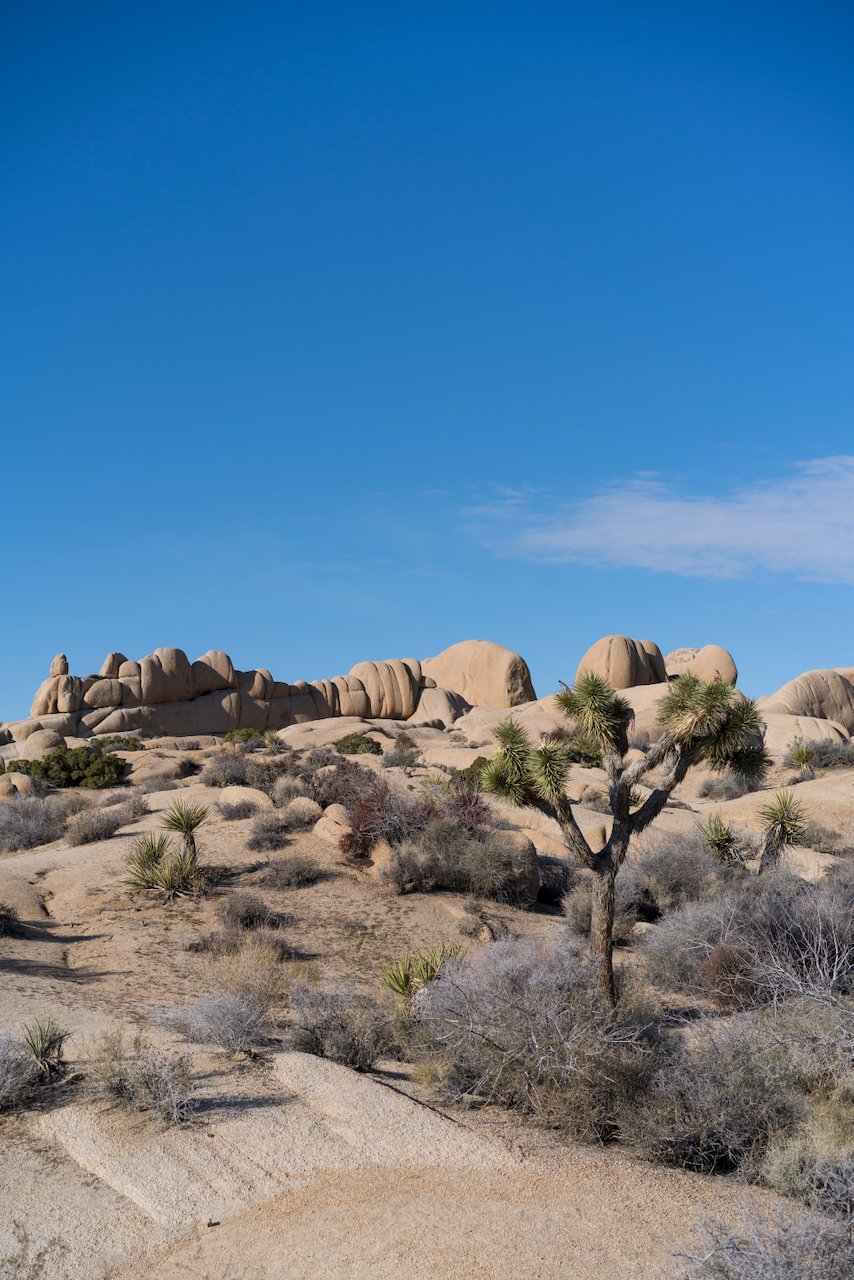
\includegraphics[width=\textwidth]{../Resource/image.png}
        \caption{Original}
        \label{fig:image-linear-bsc-original}
    \end{subfigure}
    \hfill
    \begin{subfigure}[b]{0.32\textwidth}
        \centering
        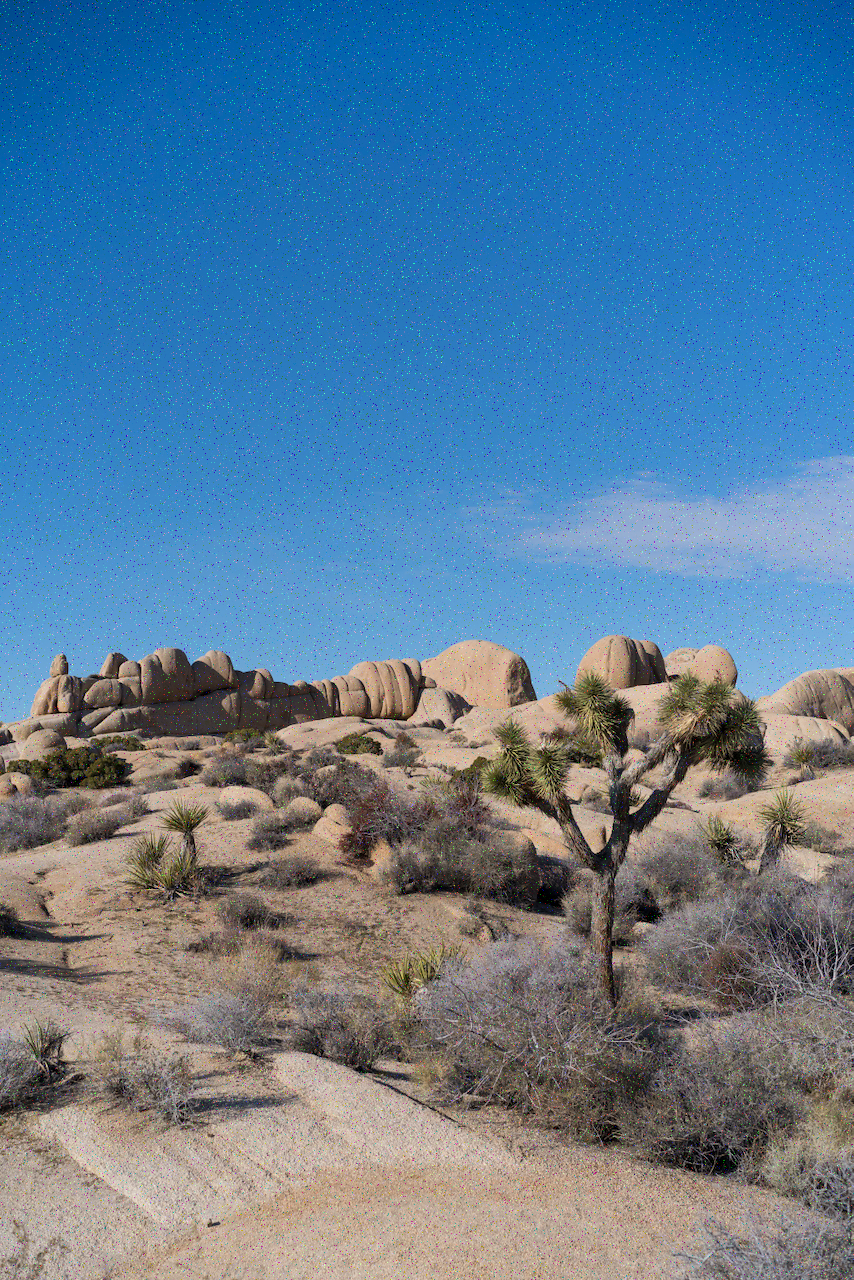
\includegraphics[width=\textwidth]{../Result/linear-bsc-output.png}
        \caption{Without correction}
        \label{fig:image-linear-bsc-no-correction}
    \end{subfigure}
    \hfill
    \begin{subfigure}[b]{0.32\textwidth}
        \centering
        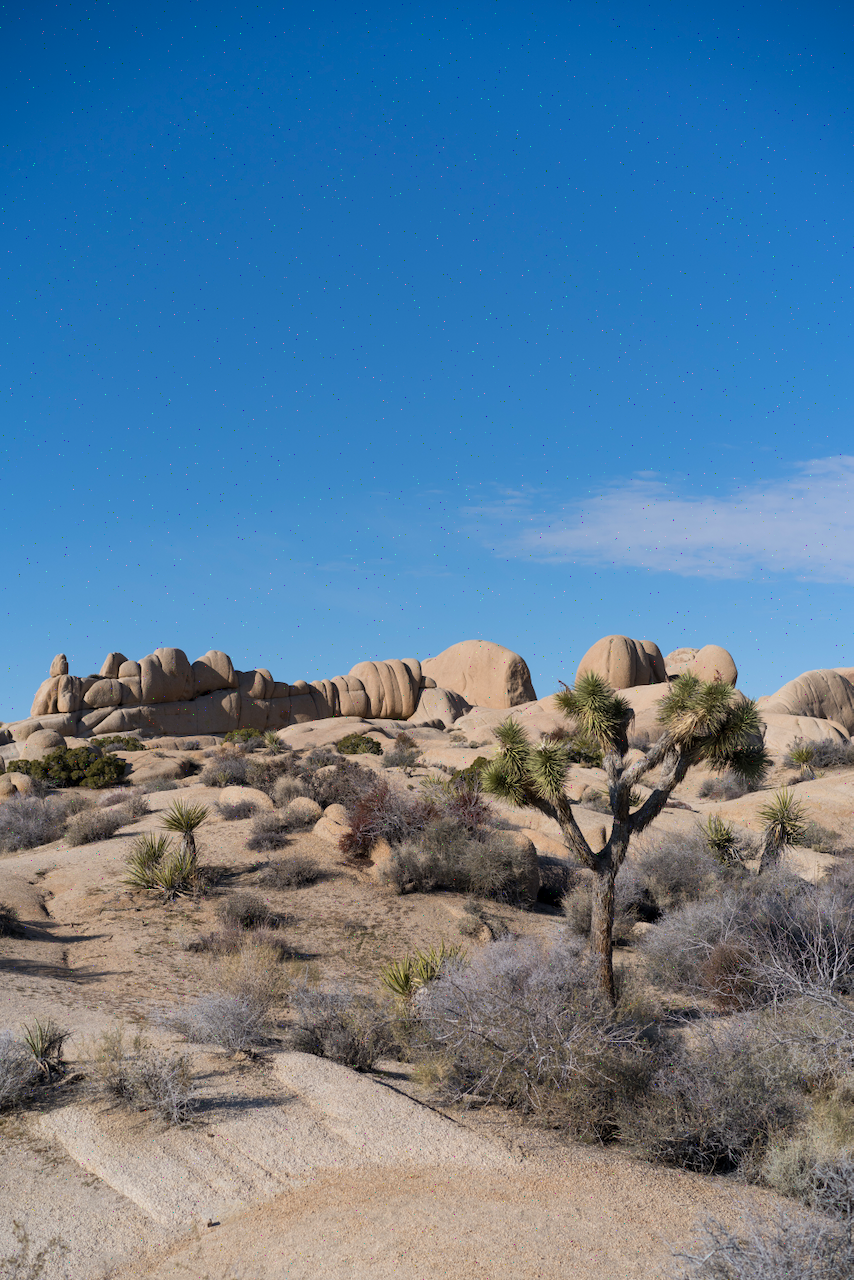
\includegraphics[width=\textwidth]{../Result/linear-bsc-output-syndrome-corrected.png}
        \caption{Corrected}
        \label{fig:image-linear-bsc-syndrome-corrected}
    \end{subfigure}
       \caption{Image encoded with Linear Hamming passed through BSC (entire)}
       \label{fig:image-linear-bsc}
\end{figure}


\begin{figure}[htb]
    \centering
    \begin{subfigure}[b]{0.32\textwidth}
        \centering
        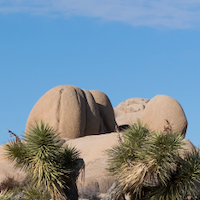
\includegraphics[width=\textwidth]{../Resource/cropped-image.png}
        \caption{Original}
        \label{fig:cropped-image-linear-bsc-original}
    \end{subfigure}
    \hfill
    \begin{subfigure}[b]{0.32\textwidth}
        \centering
        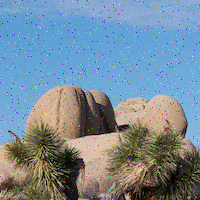
\includegraphics[width=\textwidth]{../Result/cropped-linear-bsc-output.png}
        \caption{Without correction}
        \label{fig:cropped-image-linear-bsc-no-correction}
    \end{subfigure}
    \hfill
    \begin{subfigure}[b]{0.32\textwidth}
        \centering
        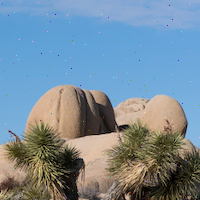
\includegraphics[width=\textwidth]{../Result/cropped-linear-bsc-output-syndrome-corrected.png}
        \caption{Corrected}
        \label{fig:cropped-image-linear-bsc-syndrome-corrected}
    \end{subfigure}
       \caption{Image encoded with Linear Hamming passed through BSC (details)}
       \label{fig:cropped-image-linear-bsc}
\end{figure}


\subsubsection{Results: audio}


\begin{figure}[htb]
    \centering
    \begin{subfigure}[b]{\textwidth}
        \centering
        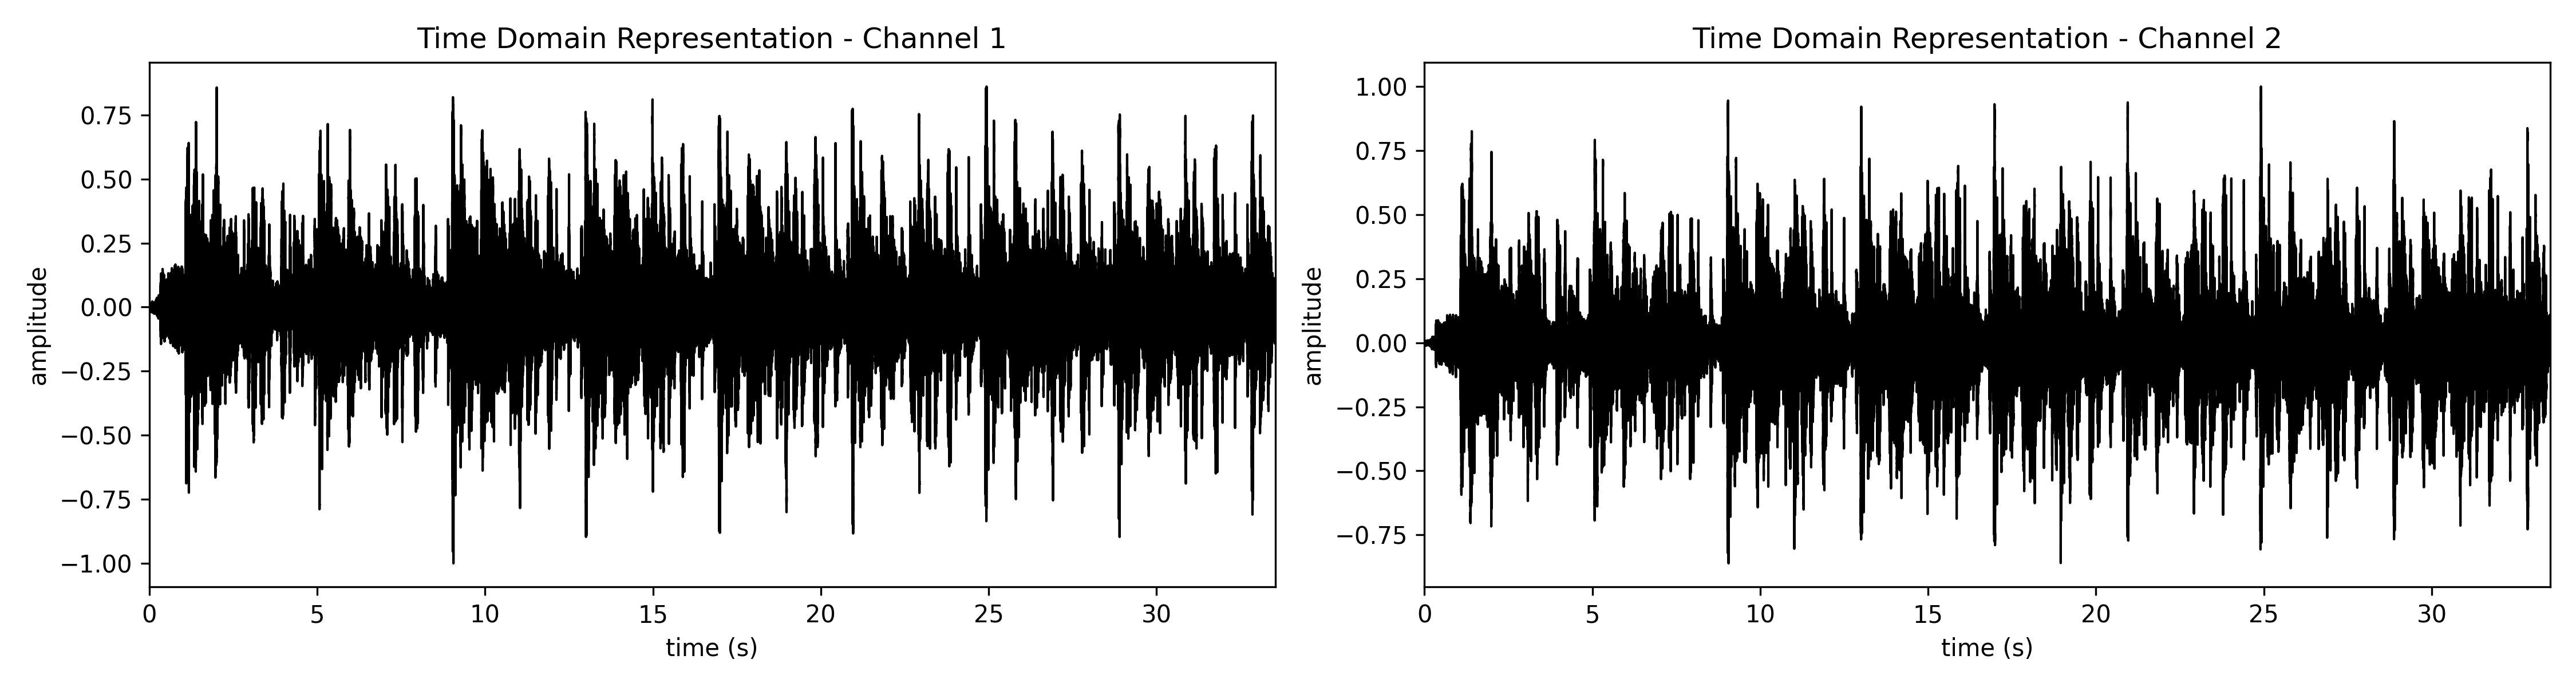
\includegraphics[width=\textwidth]{../Result/wav-time-domain-TX.png}
        \caption{Original}
        \label{fig:t-audio-linear-bsc-original}
    \end{subfigure}
    % \hfill
    \begin{subfigure}[b]{\textwidth}
        \centering
        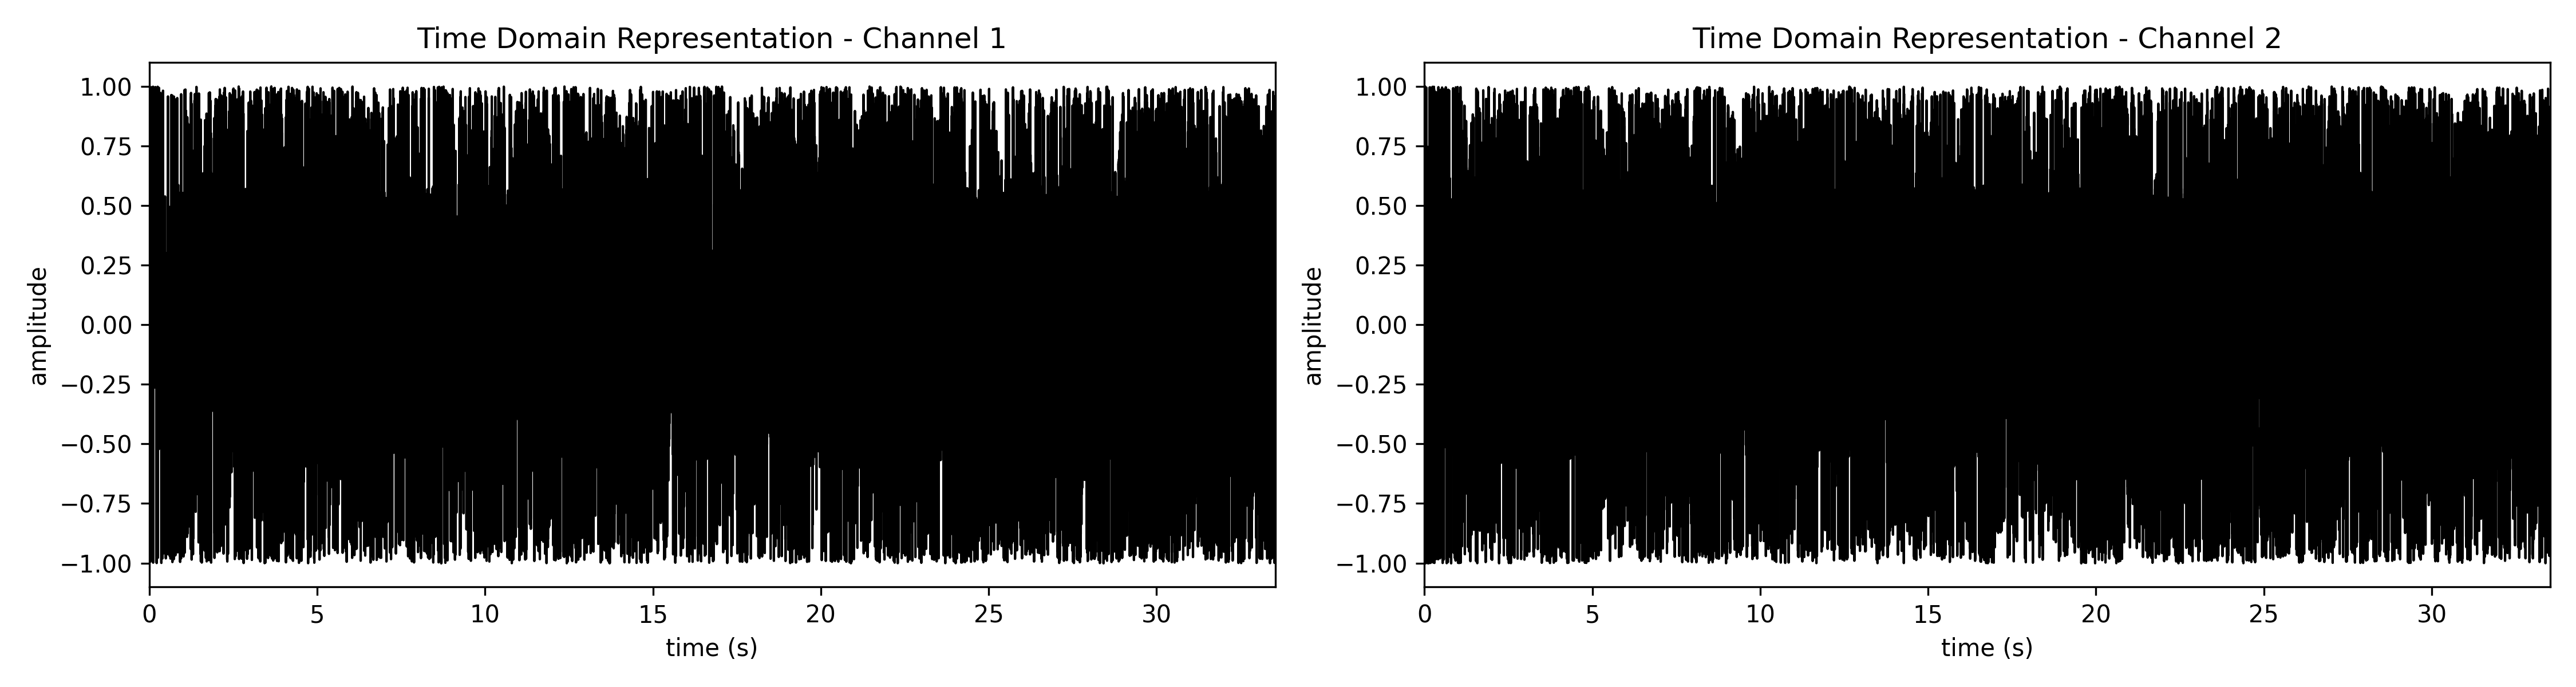
\includegraphics[width=\textwidth]{../Result/linear-bsc-wav-time-domain-RX.png}
        \caption{Without correction}
        \label{fig:t-audio-linear-bsc-no-correction}
    \end{subfigure}
    % \hfill
    \begin{subfigure}[b]{\textwidth}
        \centering
        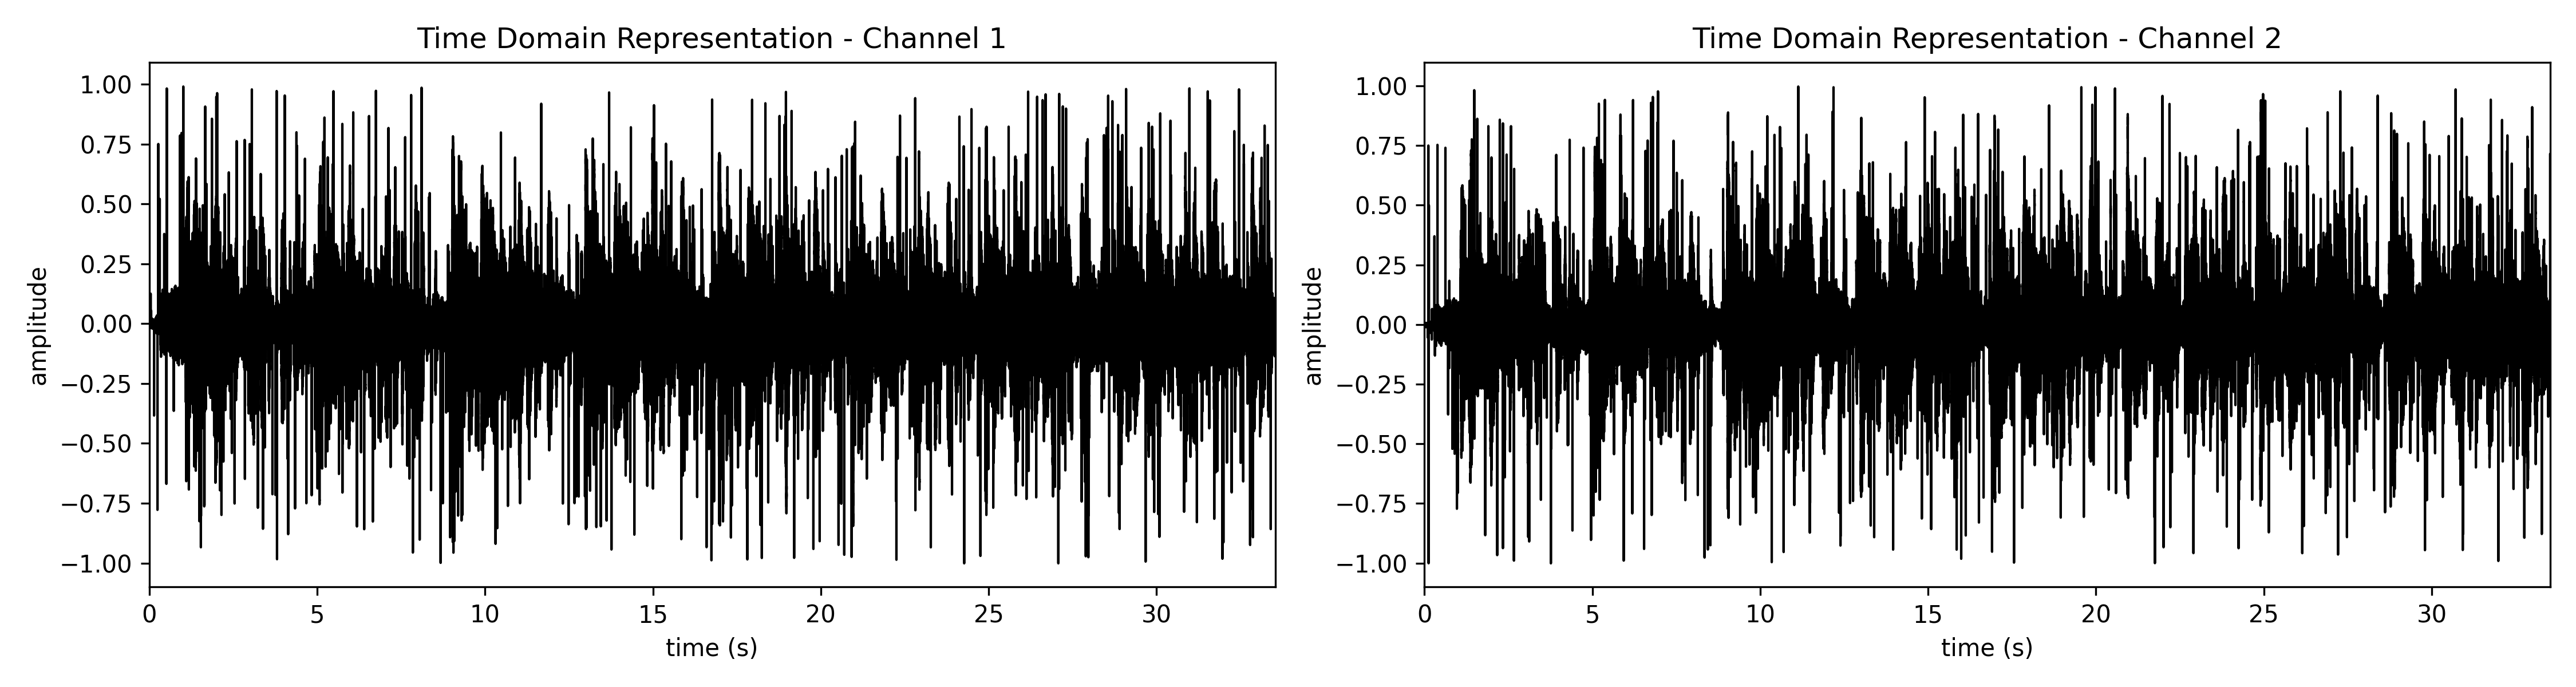
\includegraphics[width=\textwidth]{../Result/linear-bsc-wav-time-domain-RX-syndrome-corrected.png}
        \caption{Corrected}
        \label{fig:t-audio-linear-bsc-syndrome-syndrome-corrected}
    \end{subfigure}
       \caption{Audio encoded with Linear Hamming passed through BSC}
       \label{fig:t-audio-linear-bsc}
\end{figure}


\begin{figure}[htb]
    \centering
    \begin{subfigure}[b]{\textwidth}
        \centering
        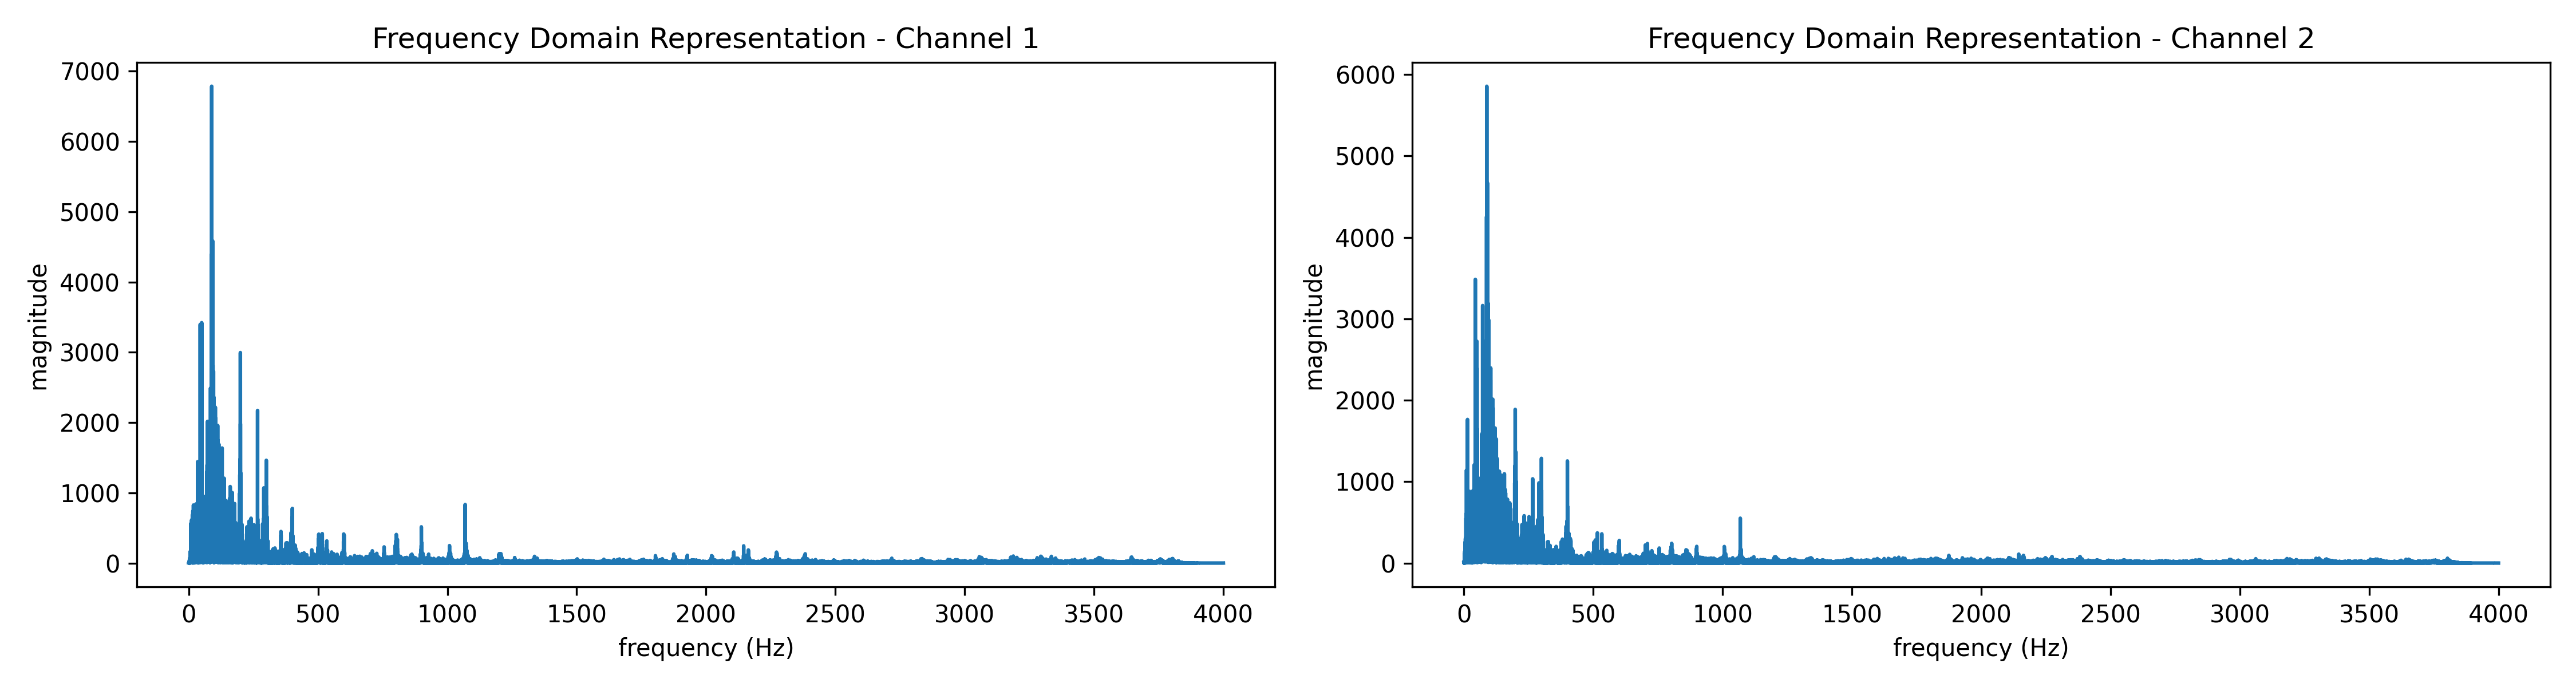
\includegraphics[width=\textwidth]{../Result/wav-frequency-domain-TX.png}
        \caption{Original}
        \label{fig:f-audio-linear-bsc-original}
    \end{subfigure}
    % \hfill
    \begin{subfigure}[b]{\textwidth}
        \centering
        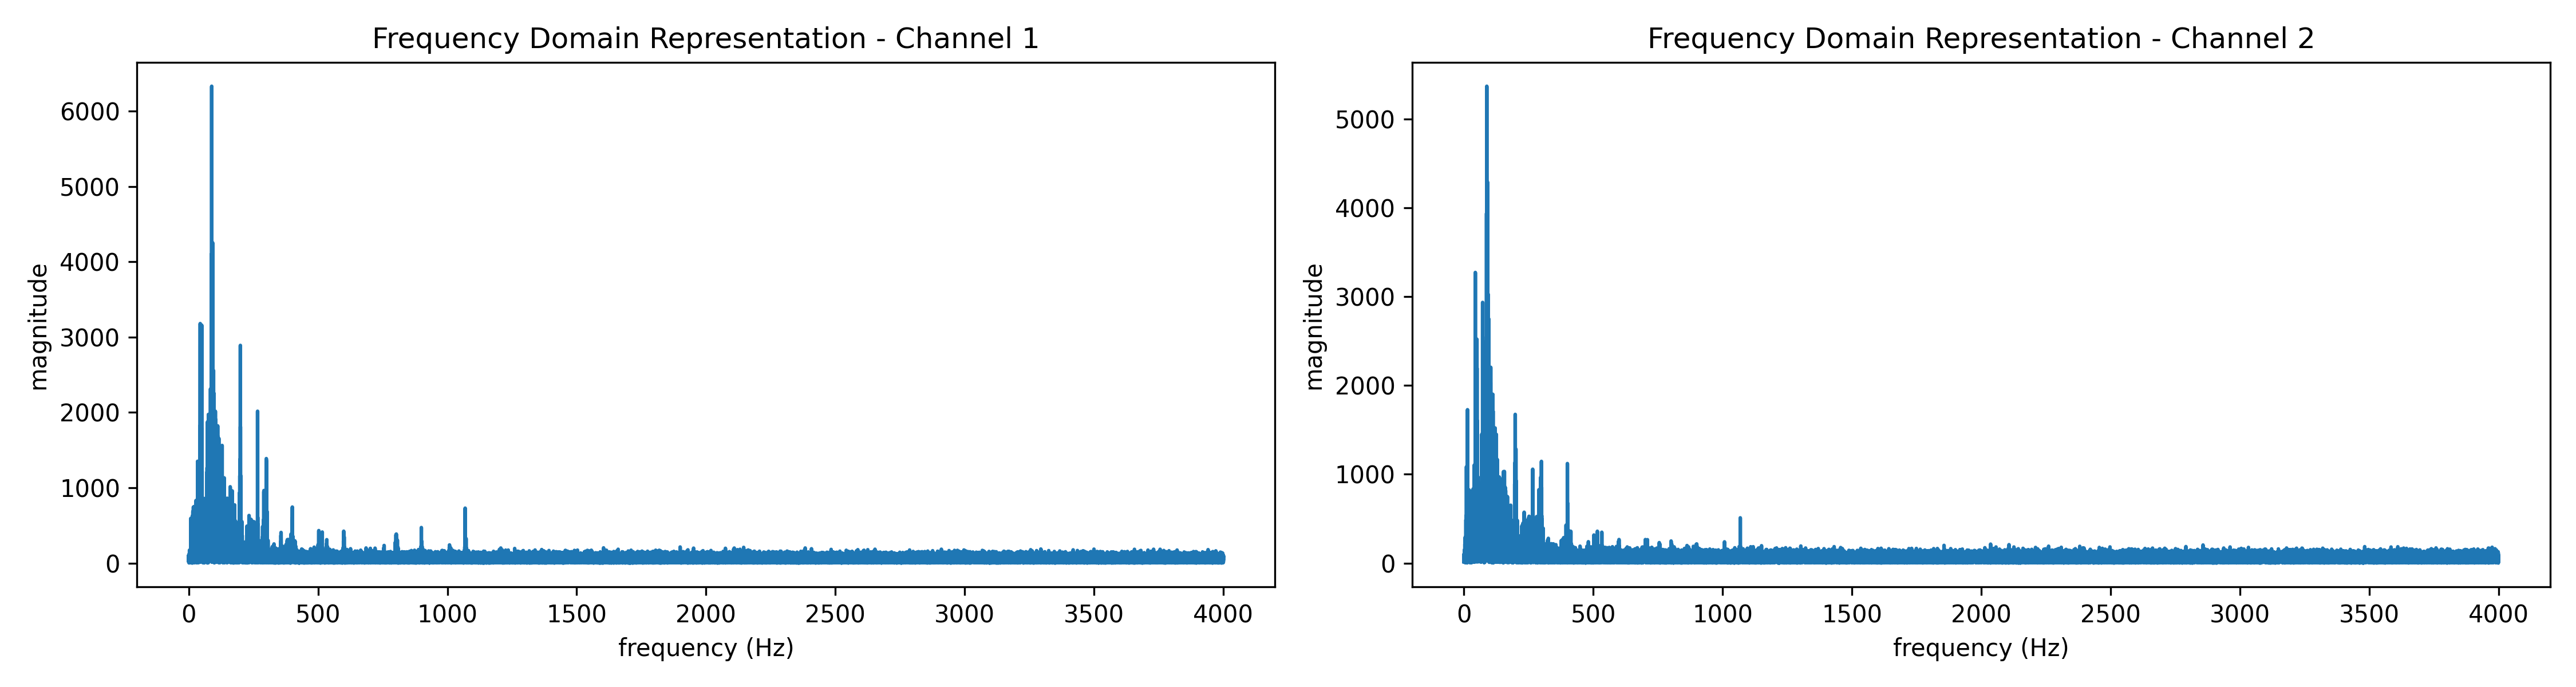
\includegraphics[width=\textwidth]{../Result/linear-bsc-wav-frequency-domain-RX.png}
        \caption{Without correction}
        \label{fig:f-audio-linear-bsc-no-correction}
    \end{subfigure}
    % \hfill
    \begin{subfigure}[b]{\textwidth}
        \centering
        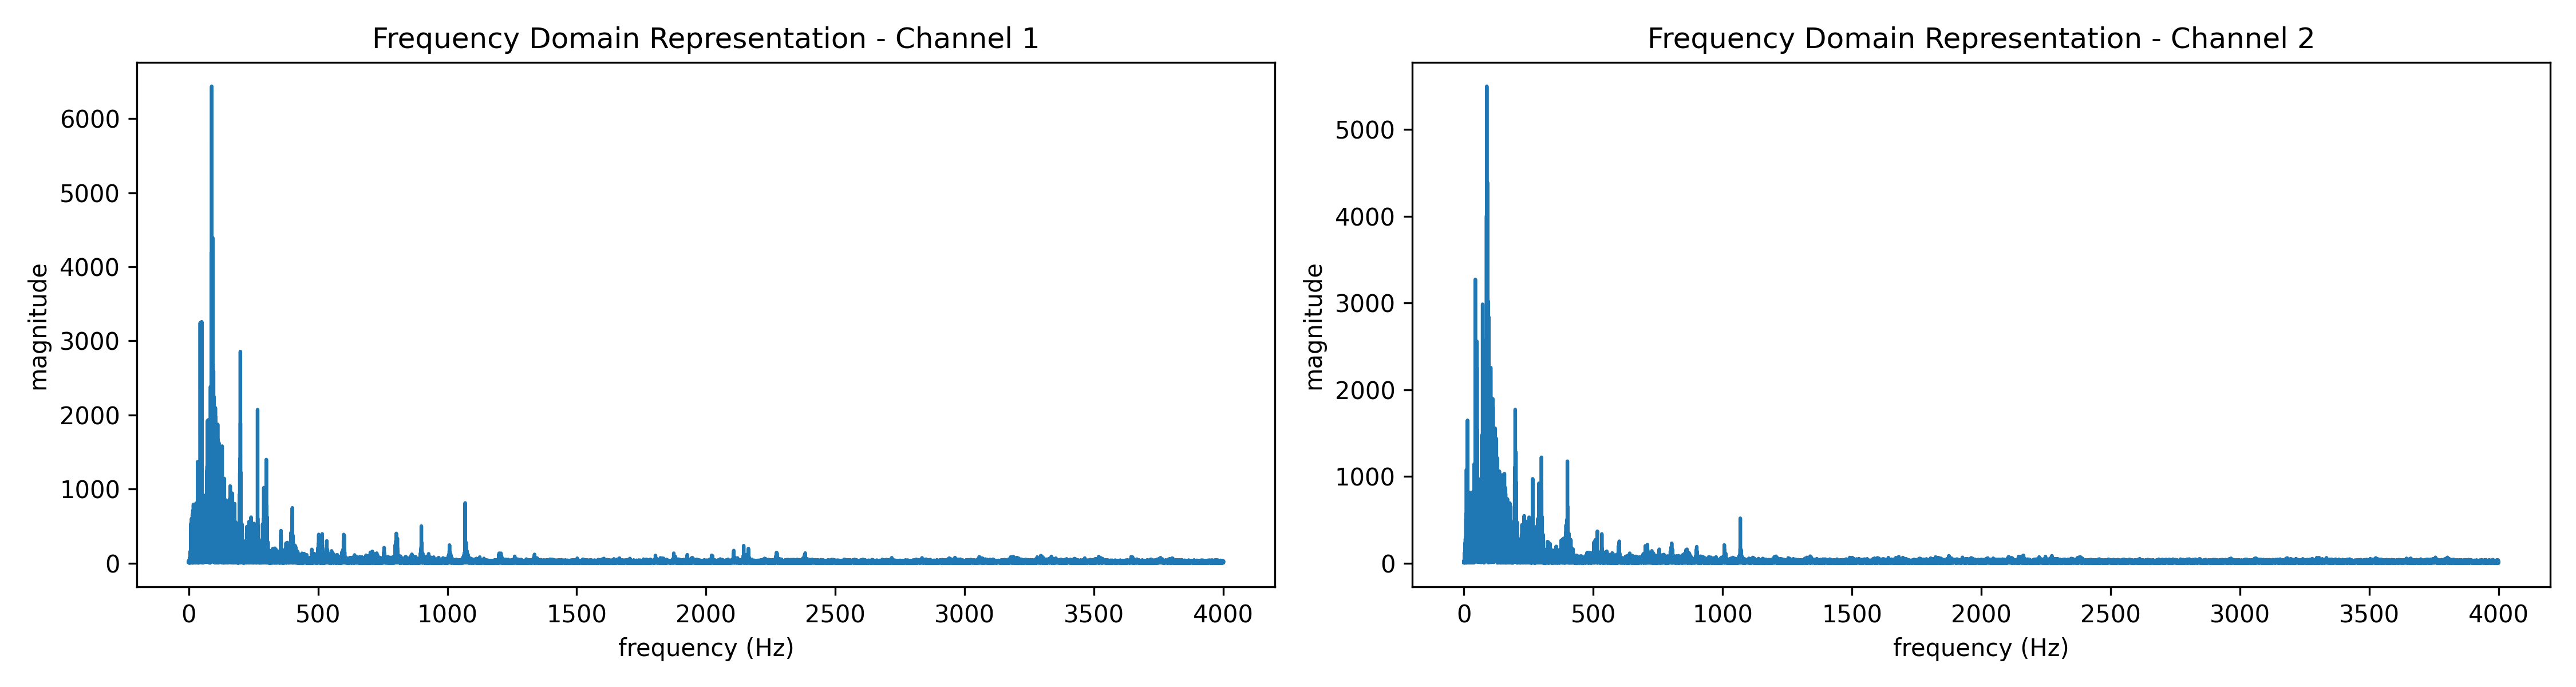
\includegraphics[width=\textwidth]{../Result/linear-bsc-wav-frequency-domain-RX-syndrome-corrected.png}
        \caption{Corrected}
        \label{fig:f-audio-linear-bsc-syndrome-corrected}
    \end{subfigure}
       \caption{Audio encoded with Linear Hamming passed through BSC}
       \label{fig:f-audio-linear-bsc}
\end{figure}


\section{$(n,k)$ Systematic Cyclic (Hamming) Code}
The $(n,k)$ Systematic Cyclic Hamming Code is a powerful and widely used error correction code (ECC) in the field of digital communications and information theory. The notation $(n,k)$ denotes that each block of the code consists of 'n' bits, where 'k' bits are the actual information or data, and the remaining 'n-k' bits are the parity or check bits used for error detection and correction.

The term "systematic" implies that the data bits remain in their original form in the encoded output, while the parity bits are appended to form the full code word. This is in contrast to non-systematic coding schemes, where the data and parity bits are intermixed.

"Cyclic" codes, meanwhile, have a key property where a cyclic shift of a code word results in another valid code word. This cyclic nature leads to efficient implementation, especially in hardware, as simple shift registers can be used.

Hamming codes, named after Richard Hamming, are a specific class of linear error-correcting codes that are renowned for their ability to correct single-bit errors in code words. They accomplish this by introducing additional parity bits that allow the identification of single-bit errors.

In the context of $(n,k)$ Systematic Cyclic Hamming Codes, the codes are designed such that any single-bit error can be detected and corrected, making them a reliable choice for environments where such errors are common and the integrity of information is paramount.


\subsection{Adjustable $(n,k)$}
\label{sec:adjustable-nk}
\textcolor{red}{TODO}

\subsection{Encoder}
The encoding process in a $(n,k)$ Systematic Cyclic Code involves the multiplication of a $k$-bit message vector with a generator matrix. The generator matrix for a $(n,k)$ Cyclic Hamming Code, in its systematic form, is given as:
% \begin{equation*}
%     G = 
%     \begin{bmatrix}
%         1 & 1 & 0 & 0 & 1 & 0 & 0 & 0 & 0 & 0 & 0 & 0 & 0 & 0 & 0 \\
%         0 & 1 & 1 & 0 & 0 & 1 & 0 & 0 & 0 & 0 & 0 & 0 & 0 & 0 & 0 \\
%         0 & 0 & 1 & 1 & 0 & 0 & 1 & 0 & 0 & 0 & 0 & 0 & 0 & 0 & 0 \\
%         1 & 1 & 0 & 1 & 0 & 0 & 0 & 1 & 0 & 0 & 0 & 0 & 0 & 0 & 0 \\
%         1 & 0 & 1 & 0 & 0 & 0 & 0 & 0 & 1 & 0 & 0 & 0 & 0 & 0 & 0 \\
%         0 & 1 & 0 & 1 & 0 & 0 & 0 & 0 & 0 & 1 & 0 & 0 & 0 & 0 & 0 \\
%         1 & 1 & 1 & 0 & 0 & 0 & 0 & 0 & 0 & 0 & 1 & 0 & 0 & 0 & 0 \\
%         0 & 1 & 1 & 1 & 0 & 0 & 0 & 0 & 0 & 0 & 0 & 1 & 0 & 0 & 0 \\
%         1 & 1 & 1 & 1 & 0 & 0 & 0 & 0 & 0 & 0 & 0 & 0 & 1 & 0 & 0 \\
%         1 & 0 & 1 & 1 & 0 & 0 & 0 & 0 & 0 & 0 & 0 & 0 & 0 & 1 & 0 \\
%         1 & 0 & 0 & 1 & 0 & 0 & 0 & 0 & 0 & 0 & 0 & 0 & 0 & 0 & 1
%     \end{bmatrix}
% \end{equation*}
\begin{equation*}
    G = \begin{bmatrix}
        P & I_{k}
    \end{bmatrix}
\end{equation*}
where $I_k$ represents a $k$ by $k$ identity matrix, and $P$ represents a $k$ by $(n-k)$ matrix for parity-check bits. 
Following is an example of the generator matrix for a $(15,11)$ Cyclic Hamming Code, which is generated with procedures in Section~\ref{sec:adjustable-nk}:
\begin{equation*}
    G = 
    \begin{bmatrix}
        1 & 1 & 0 & 0 & 1 & 0 & \cdots & 0 & 0 \\
        0 & 1 & 1 & 0 & 0 & 1 & \cdots & 0 & 0 \\
        \vdots & \vdots & \vdots & \vdots & \vdots & \vdots & \ddots & \vdots & \vdots \\
        1 & 0 & 1 & 1 & 0 & 0 & \cdots & 1 & 0 \\
        1 & 0 & 0 & 1 & 0 & 0 & \cdots & 0 & 1 \\
    \end{bmatrix}
\end{equation*}
If we denote the message vector as 
\begin{equation*}
    u =
        \begin{bmatrix}
        u_1 & u_2 & \dots & u_k 
        \end{bmatrix},
\end{equation*}
then the encoded codeword $v$ is computed by:
\begin{equation*}
    v = u \cdot G .
\end{equation*}
This multiplication produces a $n$-bit codeword, which is then ready for transmission.


\subsection{Syndrome Decoder}
\subsubsection{Text string}

\begin{table}[htb]
    \centering
    \caption{Text string encoded with Cyclic Hamming passed through BSC}
    \label{tab:text-cyclic-bsc}
    \renewcommand{\arraystretch}{1.5}
    \begin{tabulary}{\textwidth}{ |L|L|L| } 
    \hline
    \textbf{Original} & \textbf{Without correction} & \textbf{Corrected} \\
    \hline
    Hello World! EEC269A Error Correcting Code Demo & H\textcolor{red}{u,}lo World! EEC269A Error Correcti\textcolor{red}{f}g Code Demo & Hello World! EEC269A Error Correcting Code Demo \\
    \hline
    \end{tabulary}
\end{table}



\subsubsection{Image}


\begin{figure}[htb]
    \centering
    \begin{subfigure}[b]{0.32\textwidth}
        \centering
        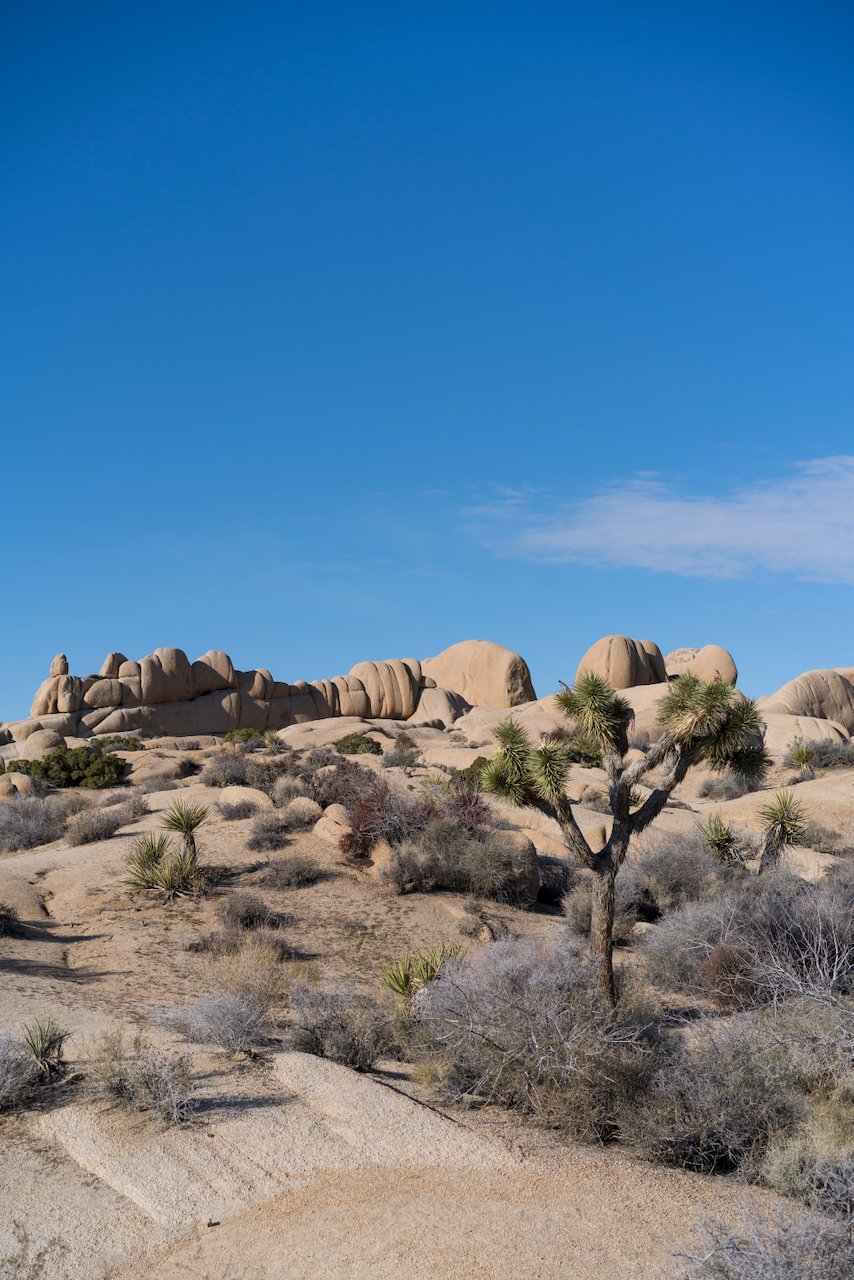
\includegraphics[width=\textwidth]{../Resource/image.png}
        \caption{Original}
        \label{fig:image-cyclic-bsc-original}
    \end{subfigure}
    \hfill
    \begin{subfigure}[b]{0.32\textwidth}
        \centering
        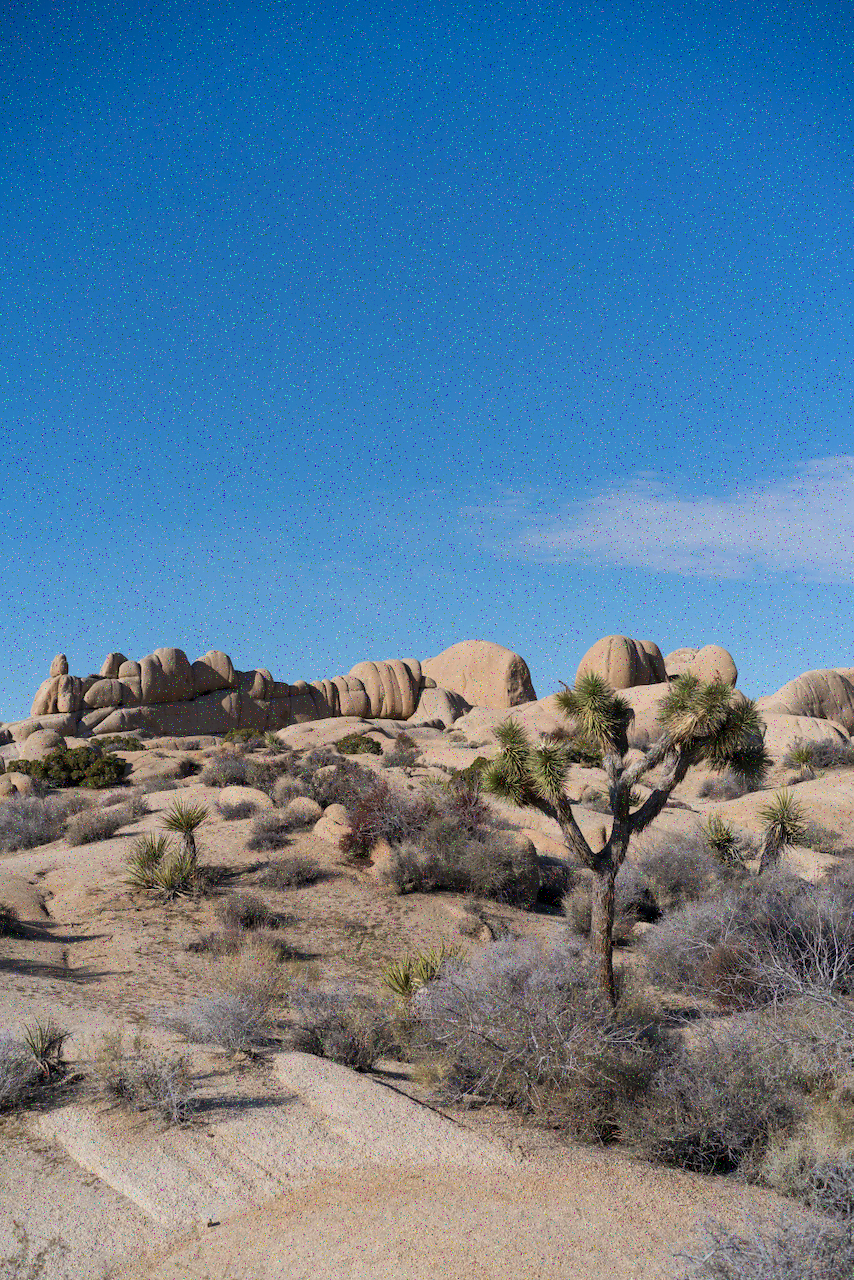
\includegraphics[width=\textwidth]{../Result/cyclic-bsc-output.png}
        \caption{Without correction}
        \label{fig:image-cyclic-bsc-no-correction}
    \end{subfigure}
    \hfill
    \begin{subfigure}[b]{0.32\textwidth}
        \centering
        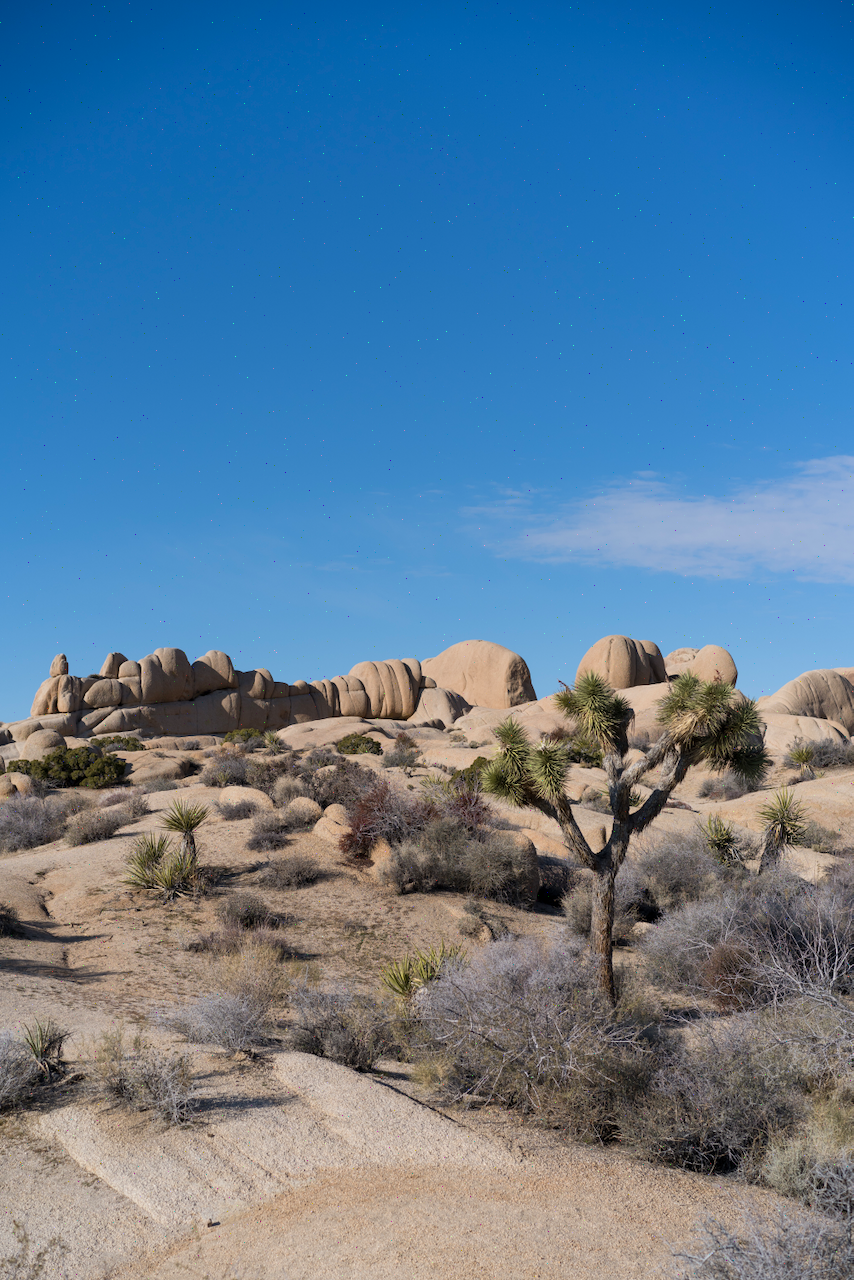
\includegraphics[width=\textwidth]{../Result/cyclic-bsc-output-syndrome-corrected.png}
        \caption{Corrected}
        \label{fig:image-cyclic-bsc-syndrome-corrected}
    \end{subfigure}
       \caption{Image encoded with Cyclic Hamming passed through BSC (entire)}
       \label{fig:image-cyclic-bsc}
\end{figure}




\begin{figure}[htb]
    \centering
    \begin{subfigure}[b]{0.32\textwidth}
        \centering
        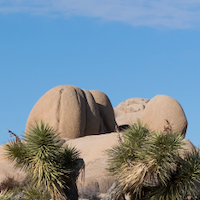
\includegraphics[width=\textwidth]{../Resource/cropped-image.png}
        \caption{Original}
        \label{fig:cropped-image-cyclic-bsc-original}
    \end{subfigure}
    \hfill
    \begin{subfigure}[b]{0.32\textwidth}
        \centering
        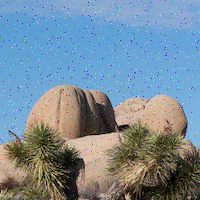
\includegraphics[width=\textwidth]{../Result/cropped-cyclic-bsc-output.png}
        \caption{Without correction}
        \label{fig:cropped-image-cyclic-bsc-no-correction}
    \end{subfigure}
    \hfill
    \begin{subfigure}[b]{0.32\textwidth}
        \centering
        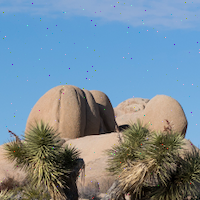
\includegraphics[width=\textwidth]{../Result/cropped-cyclic-bsc-output-syndrome-corrected.png}
        \caption{Corrected}
        \label{fig:cropped-image-cyclic-bsc-syndrome-corrected}
    \end{subfigure}
       \caption{Image encoded with Cyclic Hamming passed through BSC (details)}
       \label{fig:cropped-image-cyclic-bsc}
\end{figure}






\subsubsection{Audio}



\begin{figure}[htb]
    \centering
    \begin{subfigure}[b]{\textwidth}
        \centering
        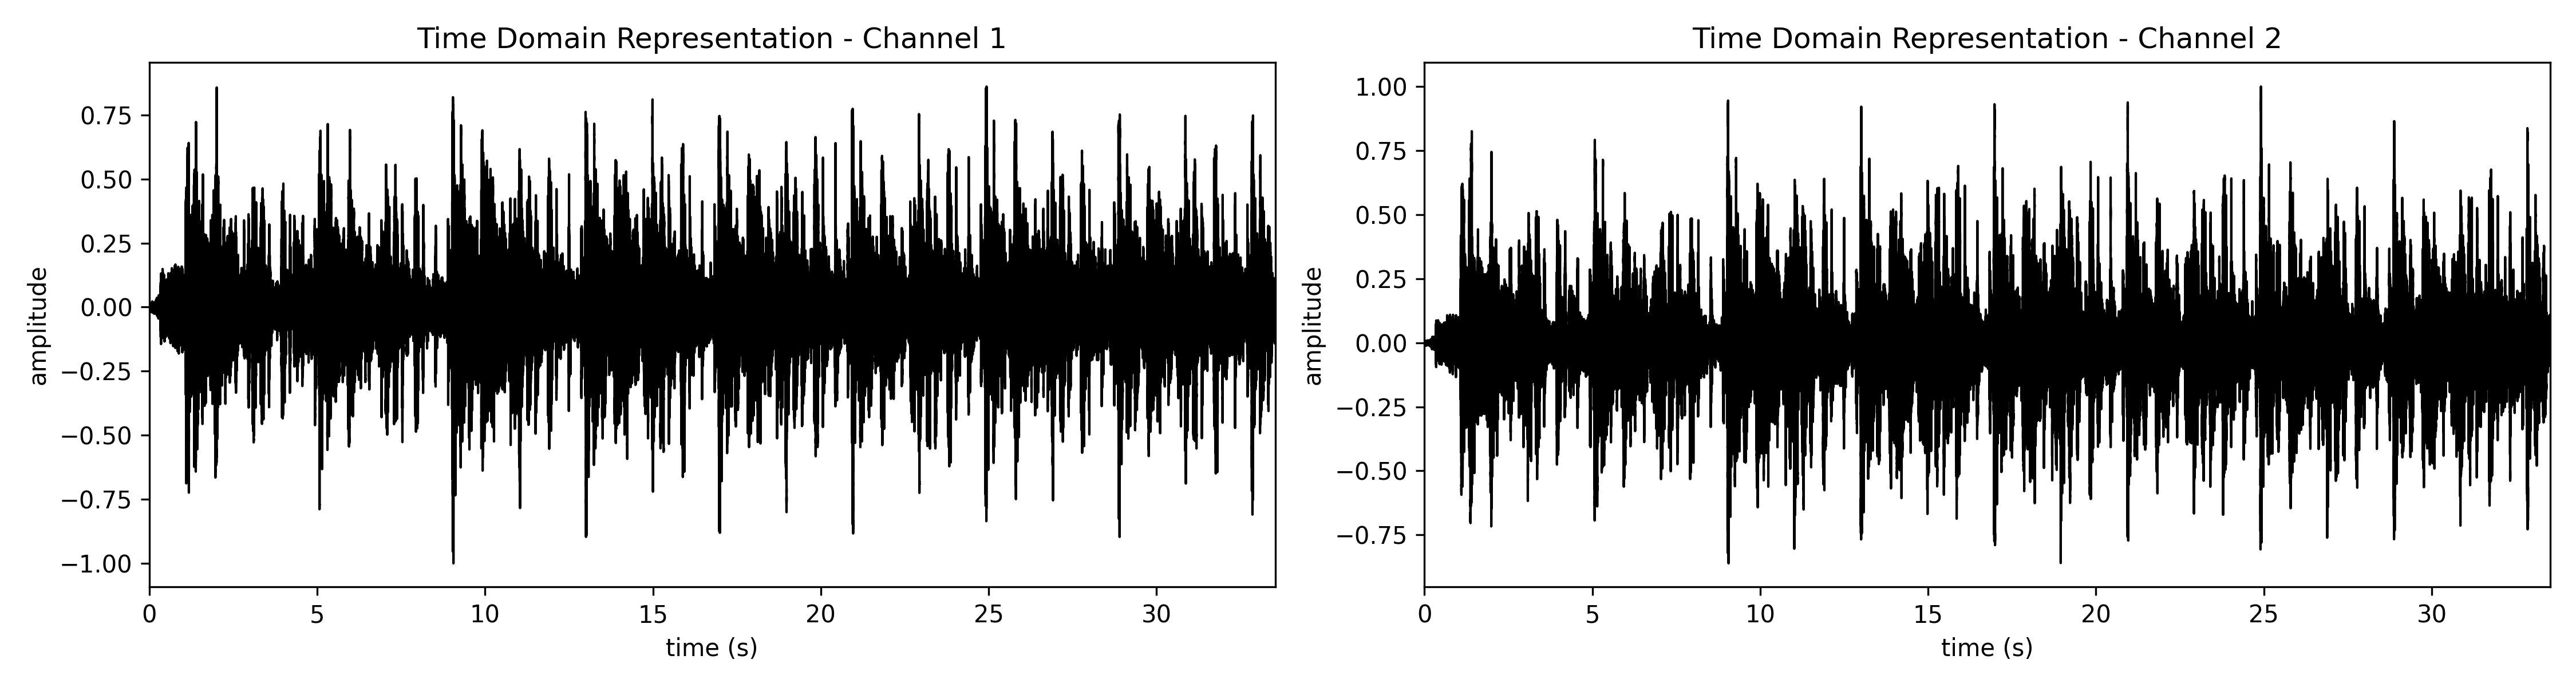
\includegraphics[width=\textwidth]{../Result/wav-time-domain-TX.png}
        \caption{Original}
        \label{fig:t-audio-cyclic-bsc-original}
    \end{subfigure}
    % \hfill
    \begin{subfigure}[b]{\textwidth}
        \centering
        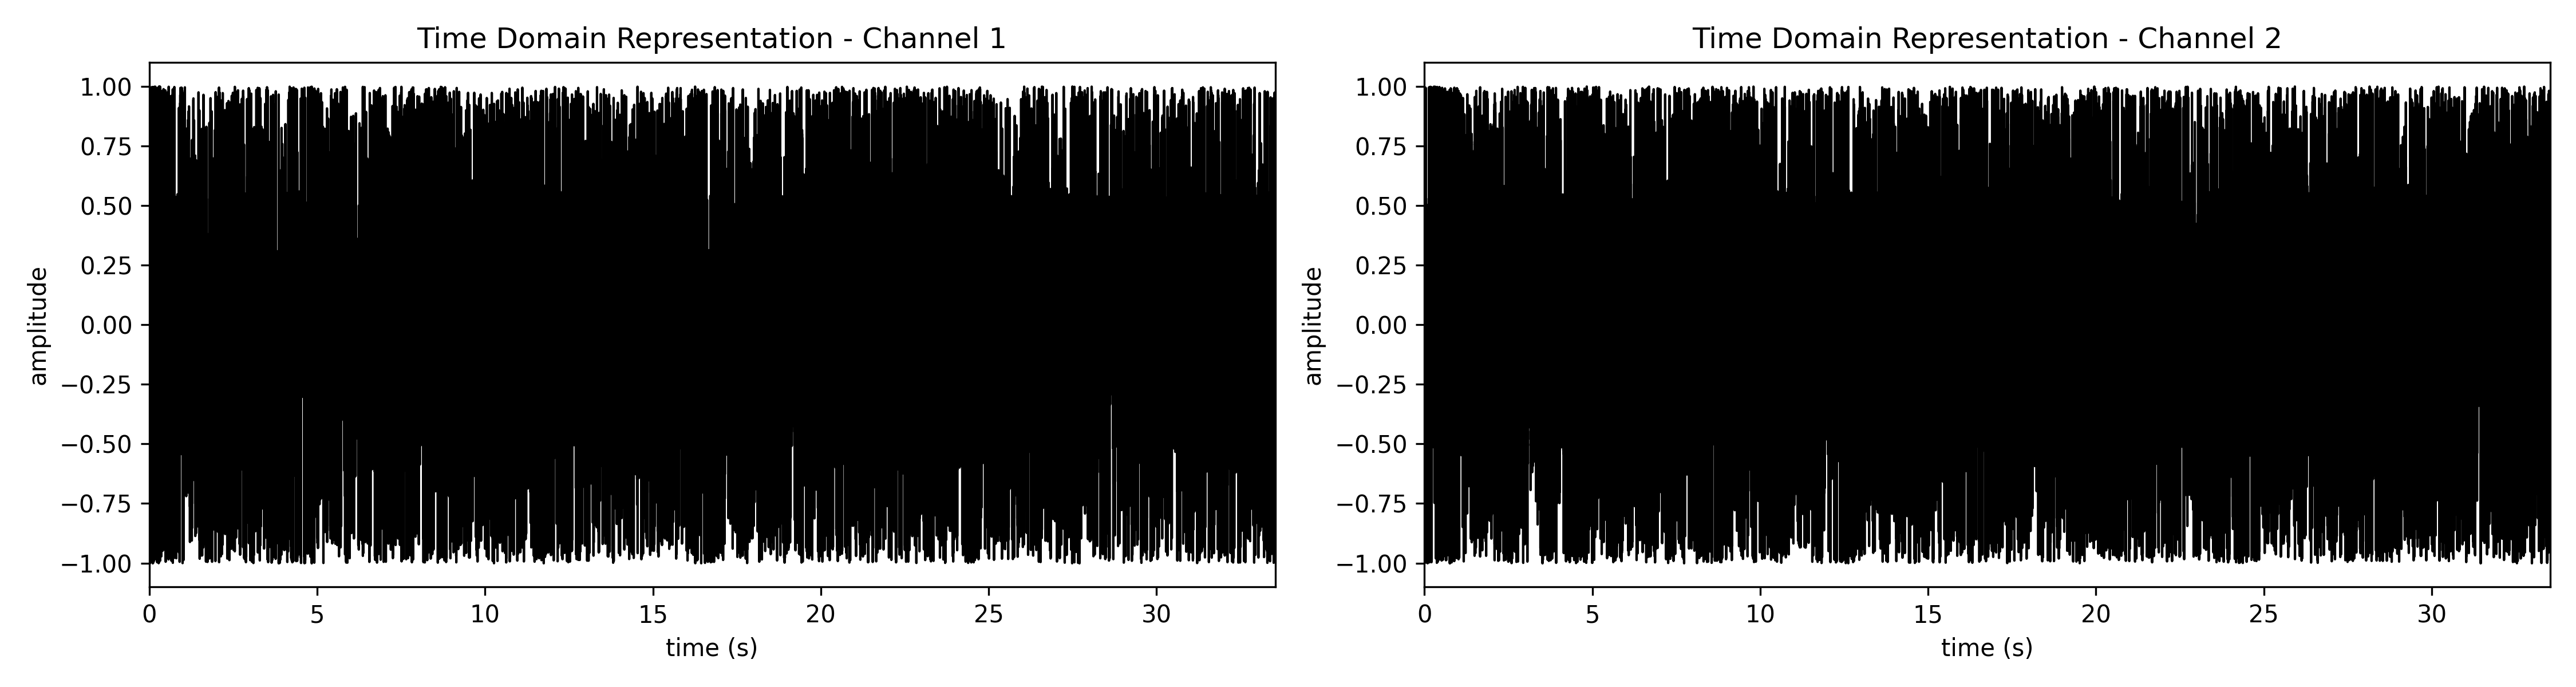
\includegraphics[width=\textwidth]{../Result/cyclic-bsc-wav-time-domain-RX.png}
        \caption{Without correction}
        \label{fig:t-audio-cyclic-bsc-no-correction}
    \end{subfigure}
    % \hfill
    \begin{subfigure}[b]{\textwidth}
        \centering
        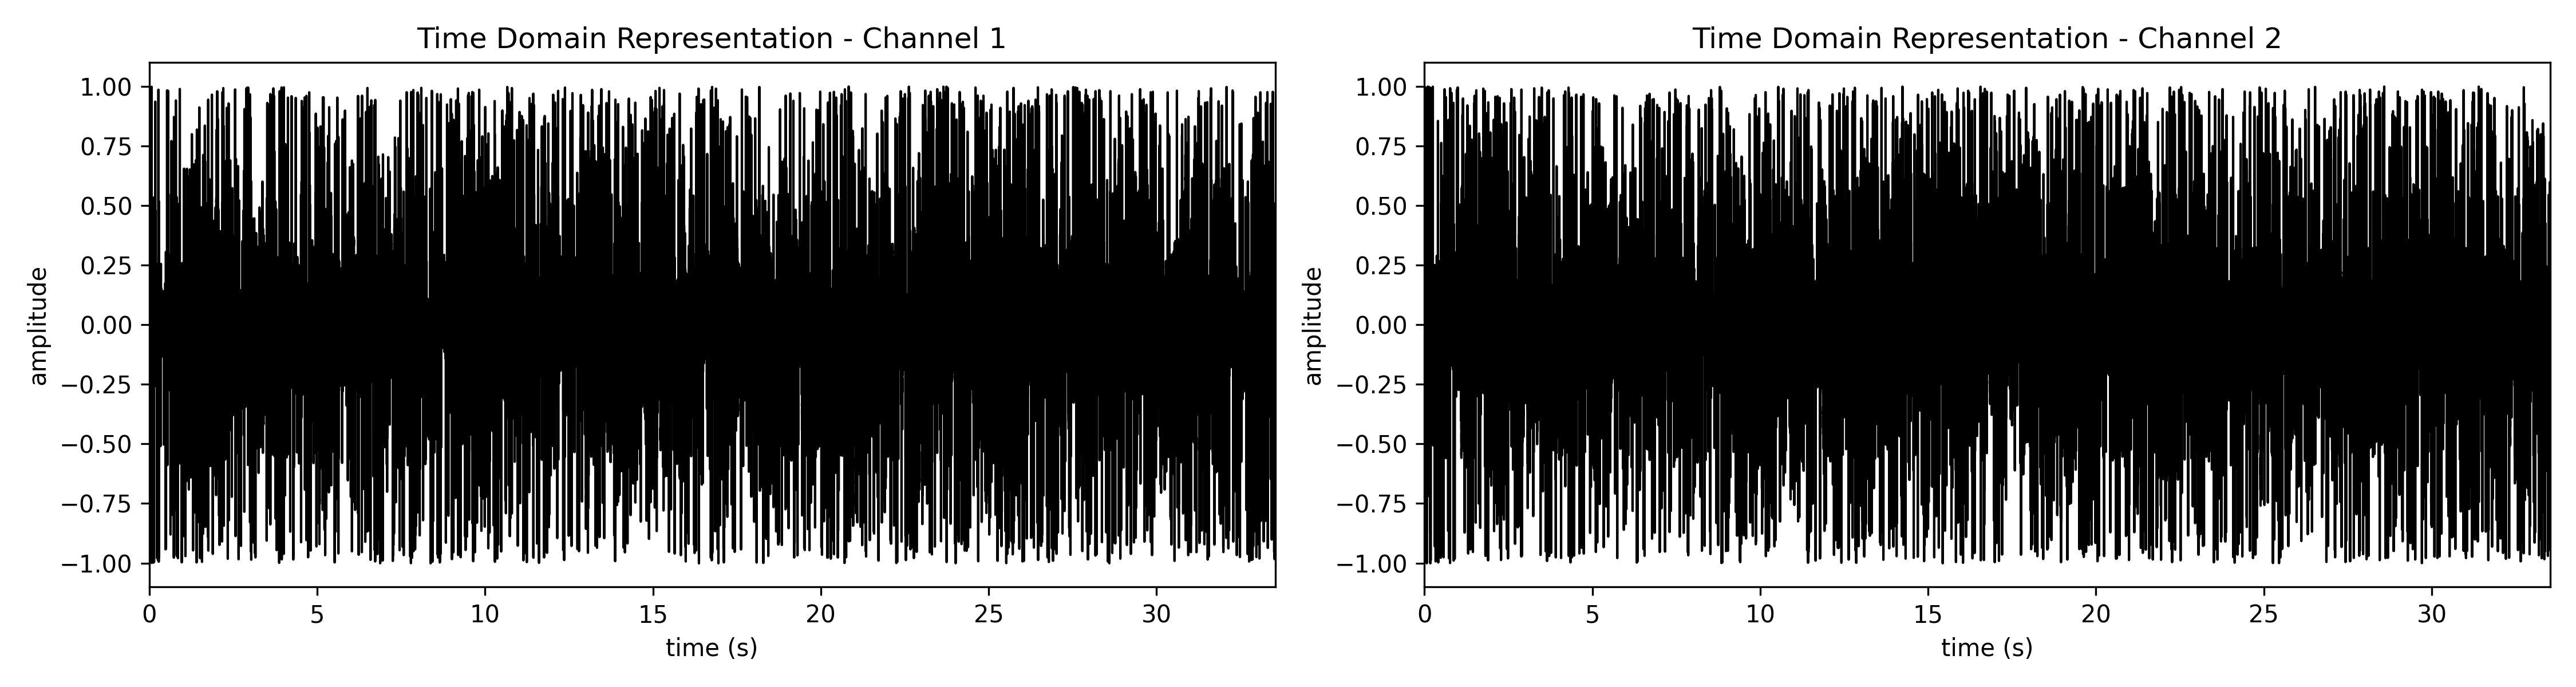
\includegraphics[width=\textwidth]{../Result/cyclic-bsc-wav-time-domain-RX-syndrome-corrected.png}
        \caption{Corrected}
        \label{fig:t-audio-cyclic-bsc-syndrome-syndrome-corrected}
    \end{subfigure}
       \caption{Audio encoded with Cyclic Hamming passed through BSC}
       \label{fig:t-audio-cyclic-bsc}
\end{figure}



\begin{figure}[htb]
    \centering
    \begin{subfigure}[b]{\textwidth}
        \centering
        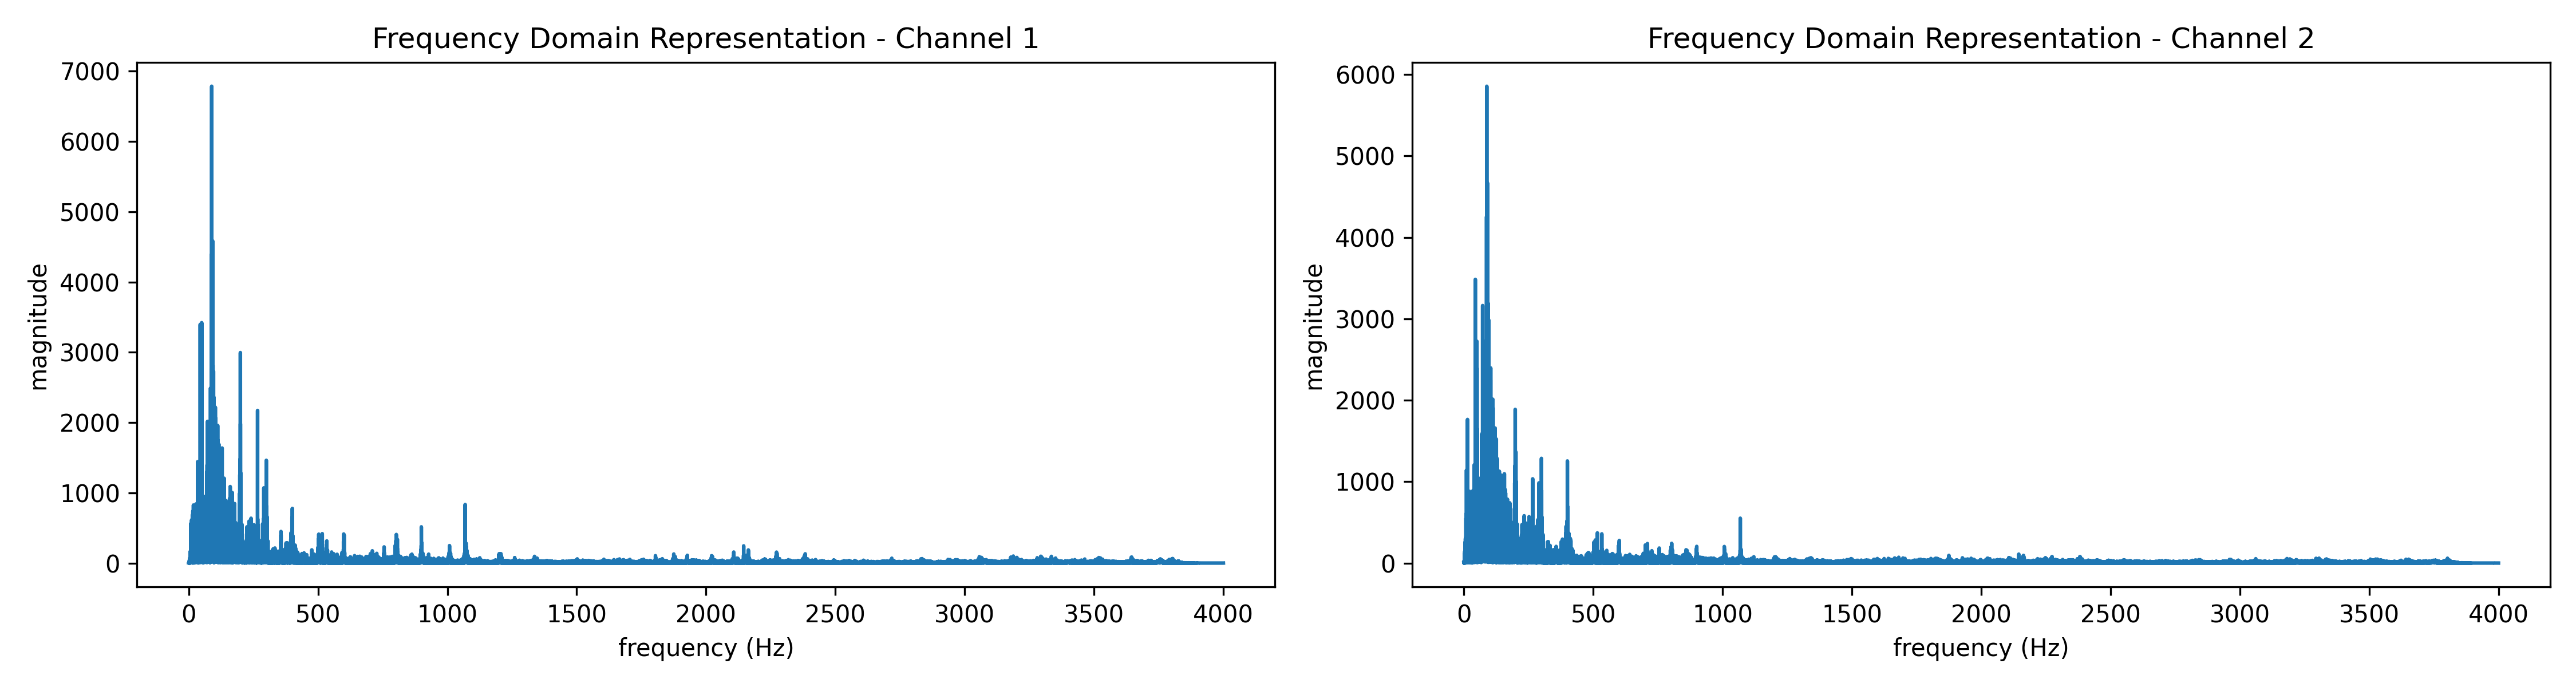
\includegraphics[width=\textwidth]{../Result/wav-frequency-domain-TX.png}
        \caption{Original}
        \label{fig:f-audio-cyclic-bsc-original}
    \end{subfigure}
    % \hfill
    \begin{subfigure}[b]{\textwidth}
        \centering
        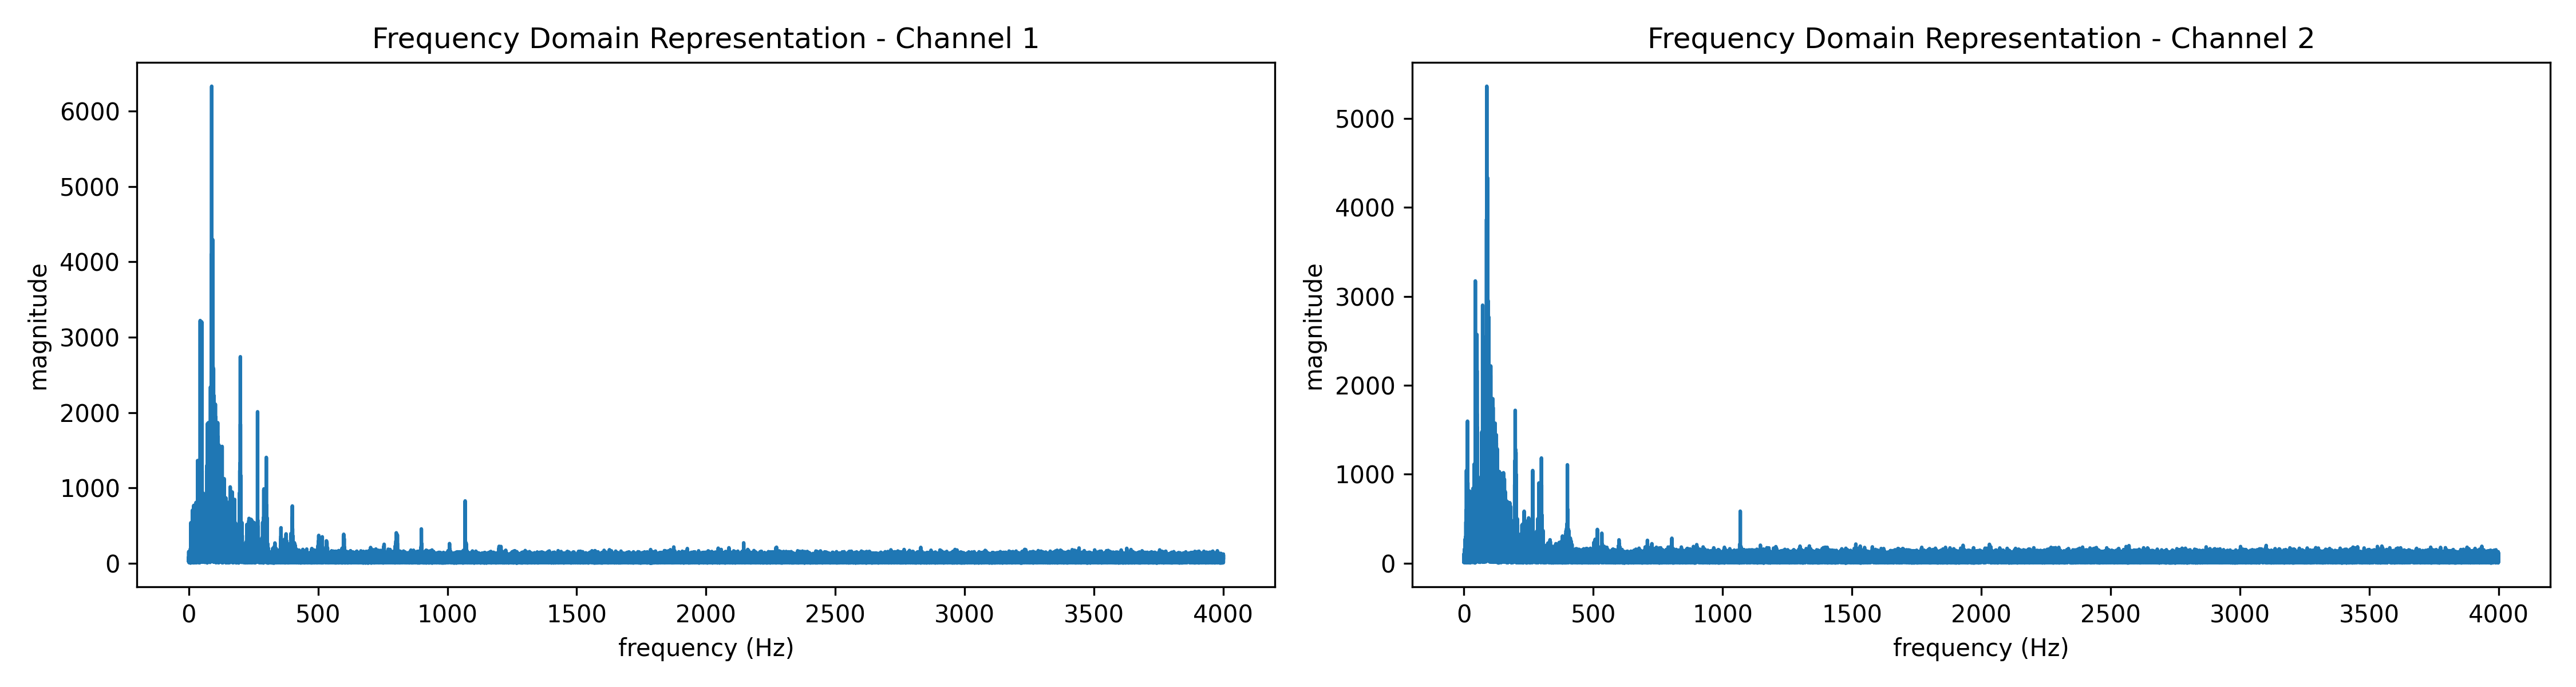
\includegraphics[width=\textwidth]{../Result/cyclic-bsc-wav-frequency-domain-RX.png}
        \caption{Without correction}
        \label{fig:f-audio-cyclic-bsc-no-correction}
    \end{subfigure}
    % \hfill
    \begin{subfigure}[b]{\textwidth}
        \centering
        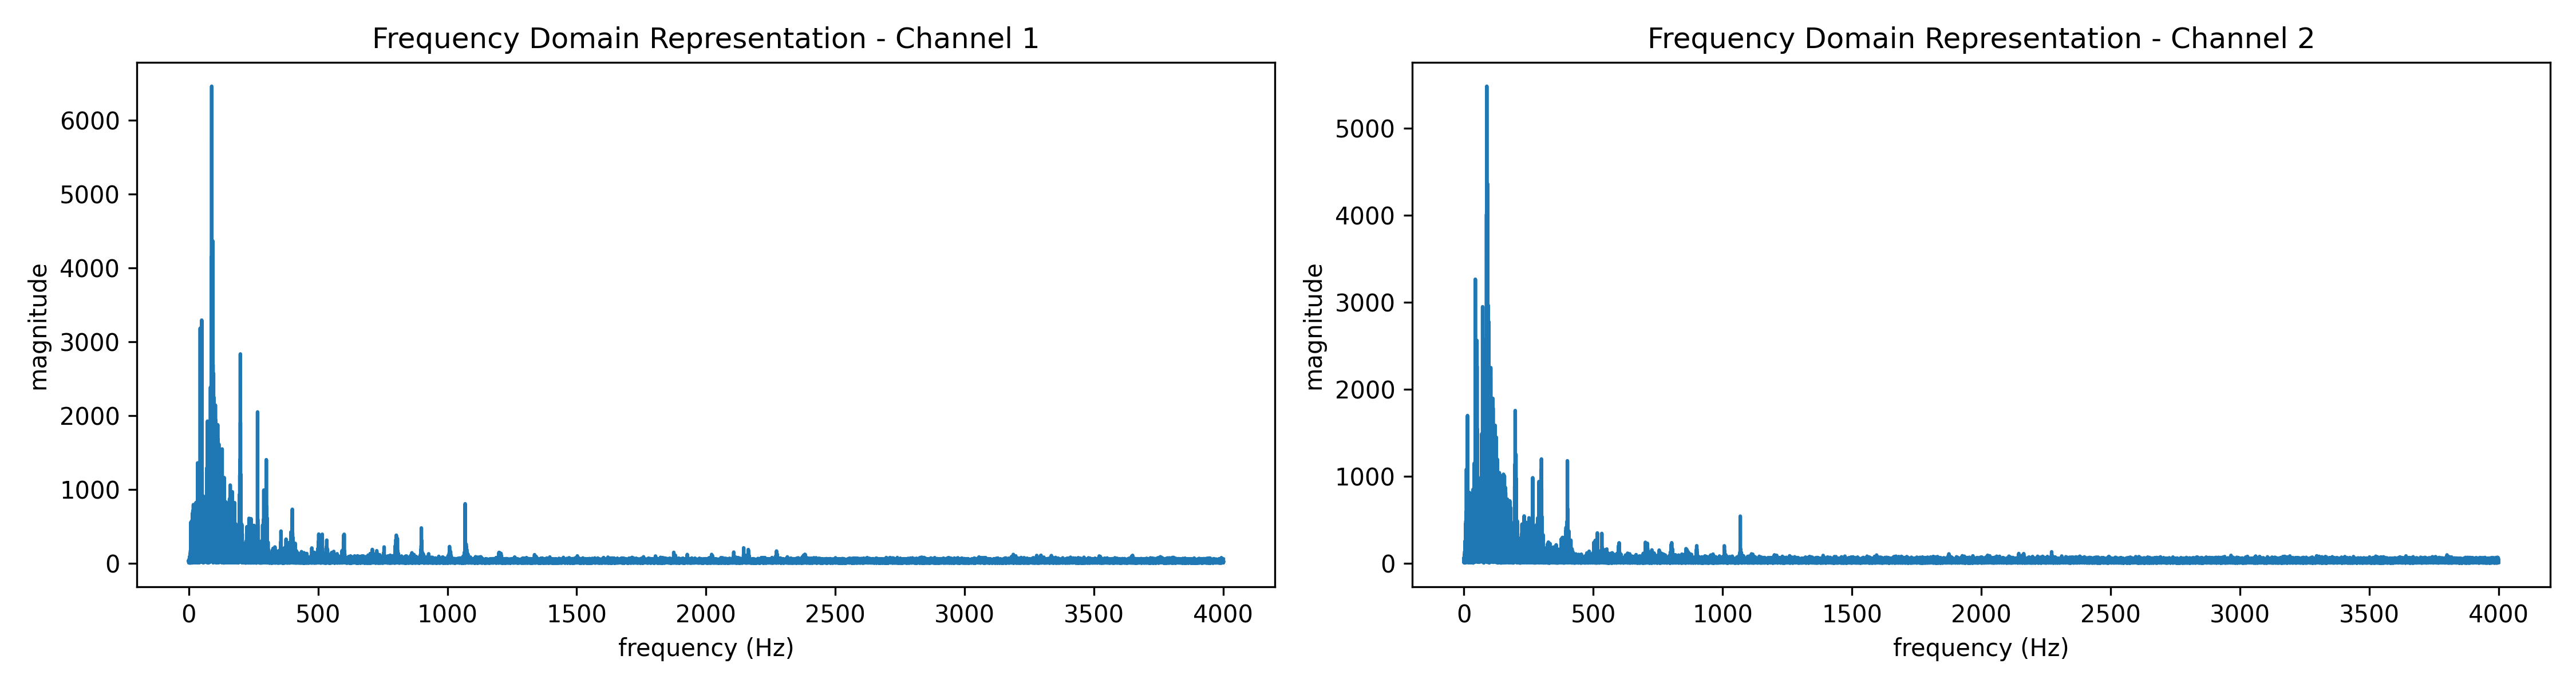
\includegraphics[width=\textwidth]{../Result/cyclic-bsc-wav-frequency-domain-RX-syndrome-corrected.png}
        \caption{Corrected}
        \label{fig:f-audio-cyclic-bsc-syndrome-corrected}
    \end{subfigure}
       \caption{Audio encoded with Cyclic Hamming passed through BSC}
       \label{fig:f-audio-cyclic-bsc}
\end{figure}






\subsection{LFSR Decoder}


\newpage
\section{Appendix: Python source code}
\subsection{Source}
\label{appendix:source}
\lstinputlisting[language=Python]{../Code/source.py}

\subsection{Channel}
\label{appendix:channel}
\lstinputlisting[language=Python]{../Code/channel.py}

\subsection{Destination}
\label{appendix:destination}
\lstinputlisting[language=Python]{../Code/destination.py}

\subsection{Utilities}
\label{appendix:utils}
\lstinputlisting[language=Python]{../Code/Utils/polyTools.py}
\lstinputlisting[language=Python]{../Code/Utils/plot_wav.py}
\lstinputlisting[language=Python]{../Code/Utils/stat_analysis.py}

\subsection{Linear code}
\label{appendix:linear-code}
\lstinputlisting[language=Python]{../Code/linear-code.py}

\subsection{Cyclic code}
\label{appendix:cyclic-code}
\lstinputlisting[language=Python]{../Code/cyclic-code.py}


\end{document}